% Title: High-Dimensional Time Series

\documentclass[14pt]{beamer}
\usepackage{amsmath,dcolumn,xmpmulti,booktabs,mathtools,animate}
\usepackage{fancyvrb,bbding,color,graphicx,eulervm,bm,pifont,bbding,ragged2e}
\usepackage{tikz}
\usetikzlibrary{trees,shapes}
\usetikzlibrary{matrix}
\tikzstyle{line} = [draw, thick]
\usetikzlibrary{calc}
\usepackage{relsize}
\tikzset{fontscale/.style = {font=\relsize{#1}}}
\usepackage{animate}

% THEME AND FORMATTING
\usetheme{metropolis}
\usepackage{MonashWhite}
\usepackage[lf,t]{carlito}
\def\FancyVerbFormatCom{\color[RGB]{6,84,142}\relax}

\def\fullwidth#1{\vspace*{0.1cm}\par\centerline{\includegraphics[width=12.8cm]{#1}}}
\def\fullheight#1{\vspace*{0.1cm}\par\centerline{\includegraphics[height=8cm]{#1}}}
\setbeamerfont{alerted text}{series=\normalfont}


% Monash title page
\setbeamerfont{title}{series=\bfseries,parent=structure,size={\fontsize{28}{32}}}
\setbeamertemplate{title page}
{\placefig{-0.01}{-0.01}{width=1.01\paperwidth,height=1.01\paperheight}{MonashTitleSlide}
\begin{textblock}{7.5}(.8,2)\fontsize{28}{32}\sf
{\color{white}\RaggedRight\usebeamerfont{title}\par\inserttitle}
\end{textblock}
\begin{textblock}{7.5}(.8,7.3)
{\color{white}\RaggedRight{\insertauthor}\\[0.2cm]
\insertdate}
\end{textblock}}

% NEW COMMANDS
\def\biz{\begin{itemize}[<+-| alert@+>]}
\def\eiz{\end{itemize}}
\def\ben{\begin{enumerate}[<+-| alert@+>]}
\def\een{\end{enumerate}}

\newcommand{\X}{\mathbf{X}}
\newcommand{\x}{\mathbf{x}}
\renewcommand{\H}{\mathbf{H}}

% GRAPHICS PATHS
\graphicspath{{figs/}}


\AtBeginSection[] {
  \begin{frame}<beamer>%[squeeze]
	\frametitle{Outline}\fontsize{14}{15}\sf\setcounter{tocdepth}{1}\vspace*{0.6cm}
    \tableofcontents[currentsection]
  \end{frame}
}

% Some local commands
\def\pred#1#2#3{\hat{#1}_{#2|#3}}
\def\h+{h_{m}^{+}}
\def\NID{\stackrel{\mbox{\scriptsize iid}}{\sim}\mbox{N}}
\def\var{\text{Var}}
\def\E{\text{E}}
\def\damped{$_{\text{\footnotesize d}}$}
\def\logN{\text{logN}}
\def\N{\text{N}}
\newcolumntype{.}{D{.}{.}{-1}}
\def\bbeta{\bm{\beta}}
\def\by{\bm{y}}
\def\bS{\bm{S}}
\def\bJ{\bm{J}}
\def\bSigma{\bm{W}}
\def\bOmega{\bm{\Omega}}
\def\bLambda{\bm{\Lambda}}
\def\mc{\multicolumn}
\def\0{\phantom{0}}
\def\bI{\text{\rm\textbf{I}}}

\newcommand{\Var}{\text{Var}}
\newcommand{\Cov}{\text{Cov}}
\newcommand{\argmin}{{\mbox{argmin}}}
\newcommand{\diag}{{\mbox{diag}}}
\newcommand{\trace}{{\mbox{trace}}}
\def\y#1#2{\pred{y}{#1}{#2}}
\def\yhat#1#2{\hat{y}_{\text{#1},#2}}
\def\ytilde#1#2{\tilde{y}_{\text{#1},#2}}
\def\Shat#1#2#3{\hat{S}_{\text{#1},#2}^{(#3)}}
\def\bs{\bm{s}}
\def\bbeta{\bm{\beta}}
\def\hl{\color[RGB]{6,84,182}}


% META INFO
\title{High-dimensional time series analysis}
\author{Rob J Hyndman}
\date{9 April 2018}

\begin{document}

\begin{frame}[plain]
\titlepage
\end{frame}\fontsize{15}{17}\sf

\section{Visualizing many time series}


\begin{frame}{M3 competition}
\fullwidth{M3paper}
\only<2>{
\placefig{1}{4}{width=2.7cm}{SMakridakis}
\placefig{8.9}{4}{width=2.3cm}{MHibon}}
\end{frame}


\begin{frame}{How to plot lots of time series?}
\only<1>{\fullwidth{M3data1}}
\only<2>{\fullwidth{M3data2}}
\only<3>{\fullwidth{M3data3}}
\only<4>{\fullwidth{M3data4}}
\only<5>{\fullwidth{M3data5}}
\only<6>{\fullwidth{M3data10}}
\only<7>{\fullwidth{M3data20}}
\only<8>{\fullwidth{M3data30}}
\only<9>{\fullwidth{M3data40}}
\only<10>{\fullwidth{M3data50}}
\only<11>{\fullwidth{M3data100}}
\only<12>{\fullwidth{M3data200}}
\only<13>{\fullwidth{M3data500}}
%\only<14>{\fullwidth{M3data1000}}
%\only<15>{\fullwidth{M3data2000}}
\only<14>{\fullwidth{M3dataall}}
\end{frame}


\begin{frame}{Key idea}
\placefig{9.1}{.5}{width=3.6cm}{tukey}
\begin{textblock}{3}(9.7,5.4)\small\textit{John W Tukey}\end{textblock}
\begin{textblock}{8}(0.7,1.2)
\begin{alertblock}{Cognostics}
Computer-produced diagnostics\\ (Tukey and Tukey, 1985).
\end{alertblock}
\end{textblock}\pause
\vspace*{1.5cm}

\structure{Examples for time series}
\begin{itemize}
\item lag correlation
\item size and direction of trend
\item strength of seasonality
\item timing of peak seasonality
\item spectral entropy
\end{itemize}

\pause\vspace*{0.4cm}
\begin{block}{}
Called ``features'' in the machine learning literature.
\end{block}

\vspace*{10cm}

\end{frame}


\begin{frame}{An STL decomposition: N2096}\vspace*{-0.2cm}
\begin{alertblock}{}
\centerline{$Y_t = S_t + T_t + R_t$\qquad $S_{t}$ is periodic with mean 0}
\end{alertblock}\vspace*{0.2cm}
\centerline{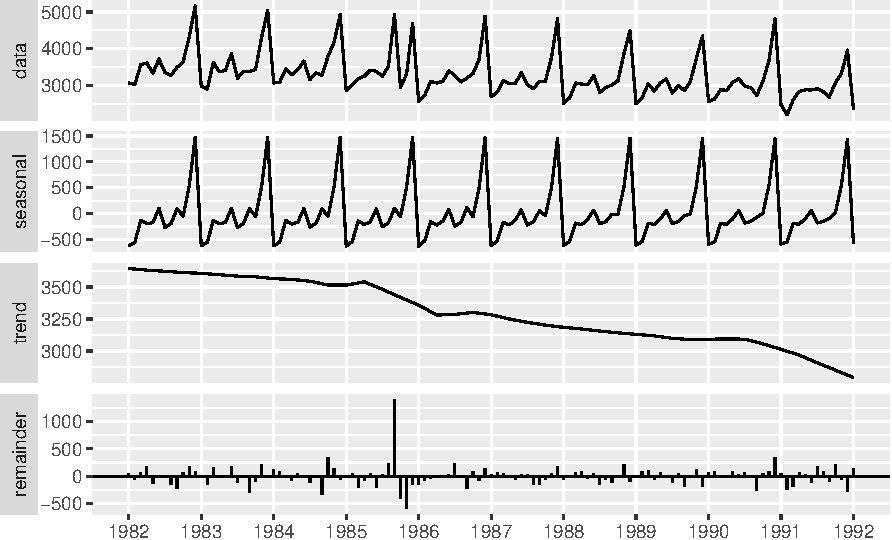
\includegraphics[width=11.5cm]{N2096}}
\end{frame}


\begin{frame}{Candidate features}\fontsize{13}{15}\sf
\begin{block}{STL decomposition}
\centerline{$Y_t = S_t + T_t + R_t$}
\end{block}\pause\vspace*{-0.2cm}
\begin{itemize}
\item Seasonal period
\item Autocorrelations of data ($Y_1,\dots,Y_T$)
\item Autocorrelations of residuals ($R_1,\dots,R_T$)
\item Strength of seasonality: $\max\left(0,1 - \frac{\Var(R_t)}{\Var(S_t+R_t)}\right)$
\item Strength of trend:  $\max\left(0,1 - \frac{\Var(R_t)}{\Var(T_t+R_t)}\right)$
\item Spectral entropy: $ H = - \int_{-\pi}^{\pi} f_y(\lambda) \log f_y(\lambda) d\lambda$, where $f_y(\lambda)$ is spectral density of $Y_t$.
\\ Low values of $H$ suggest a time series that is easier to forecast (more signal).
\item Optimal Box-Cox transformation of data
\end{itemize}
\end{frame}


\begin{frame}{Distribution of Period for M3}
\fullwidth{histPeriod}
\end{frame}

\begin{frame}{Distribution of Seasonality for M3}
\fullwidth{kdeSeasonality}
\only<2->{
\begin{textblock}{6}(0.2,3)
  \begin{block}{Low Seasonality}
    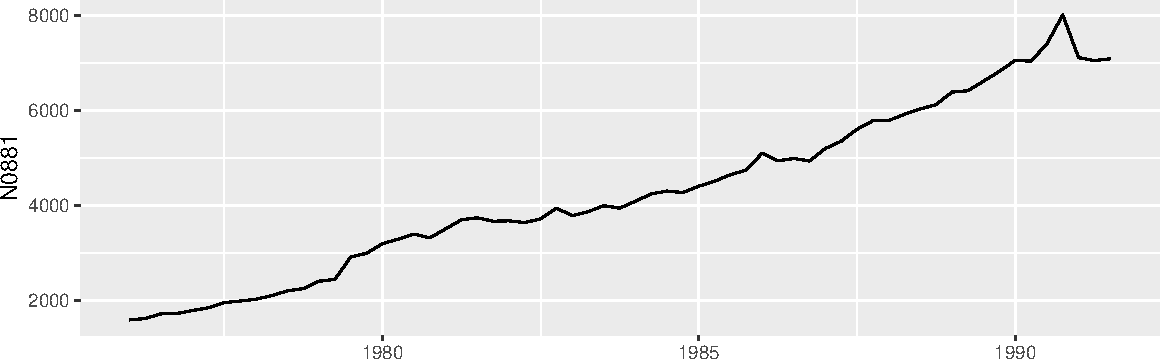
\includegraphics[width=6cm]{M3seasonLo.pdf}
  \end{block}
\end{textblock}
}
\only<3>{
\begin{textblock}{6}(6.6,3)
  \begin{block}{High Seasonality}
    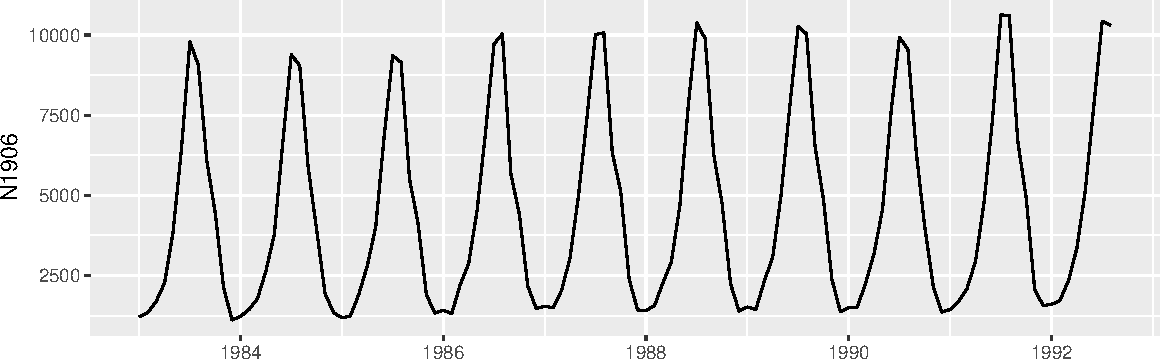
\includegraphics[width=6cm]{M3seasonHi.pdf}
  \end{block}
\end{textblock}
}
\end{frame}

\begin{frame}{Distribution of Trend for M3}
\fullwidth{kdeTrend}
\only<2->{
\begin{textblock}{6}(0.2,3)
  \begin{block}{Low Trend}
    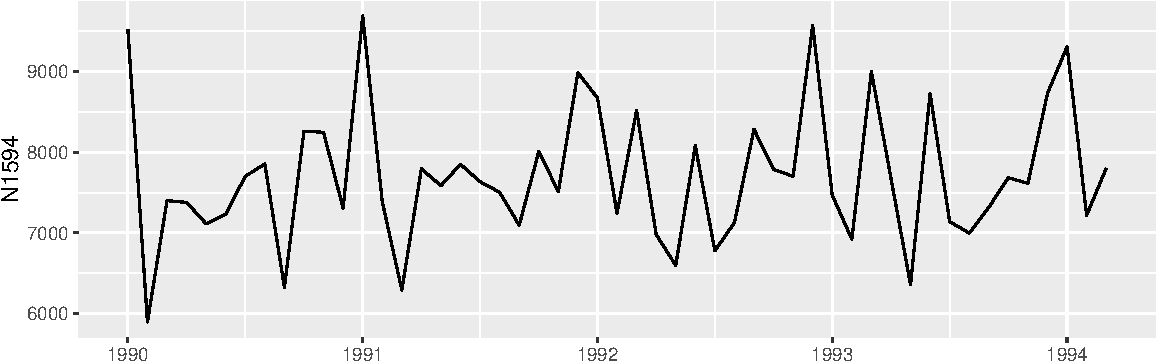
\includegraphics[width=6cm]{M3trendLo.pdf}
  \end{block}
\end{textblock}
}
\only<3>{
\begin{textblock}{6}(6.6,3)
  \begin{block}{High Trend}
    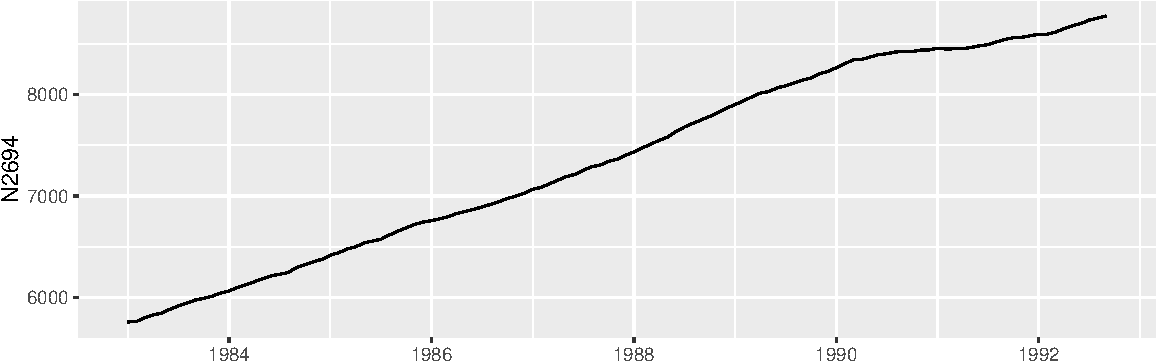
\includegraphics[width=6cm]{M3trendHi.pdf}
  \end{block}
\end{textblock}
}
\end{frame}

\begin{frame}{Distribution of residual ACF1 for M3}
\fullwidth{kdeResidACF}
\only<2->{
\begin{textblock}{6}(0.2,3)
  \begin{block}{Low ACF1}
    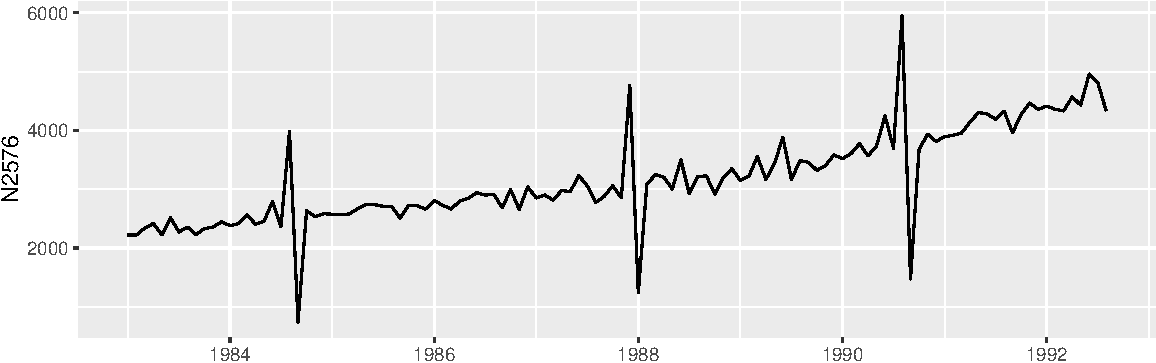
\includegraphics[width=6cm]{M3acfLo.pdf}
  \end{block}
\end{textblock}
}
\only<3>{
\begin{textblock}{6}(6.6,3)
  \begin{block}{High ACF1}
    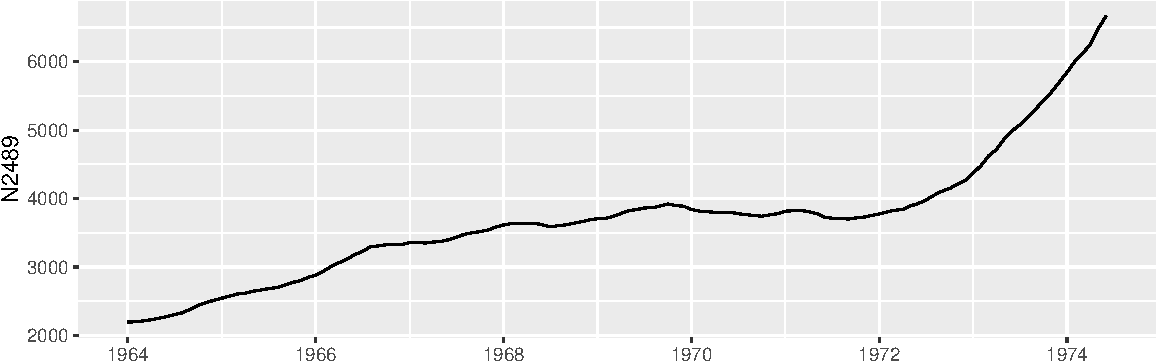
\includegraphics[width=6cm]{M3acfHi.pdf}
  \end{block}
\end{textblock}
}\end{frame}

\begin{frame}{Distribution of Spectral Entropy for M3}
\fullwidth{kdeSpectralEntropy}
\only<2->{
\begin{textblock}{6}(0.2,3)
  \begin{block}{Low Spectral Entropy}
    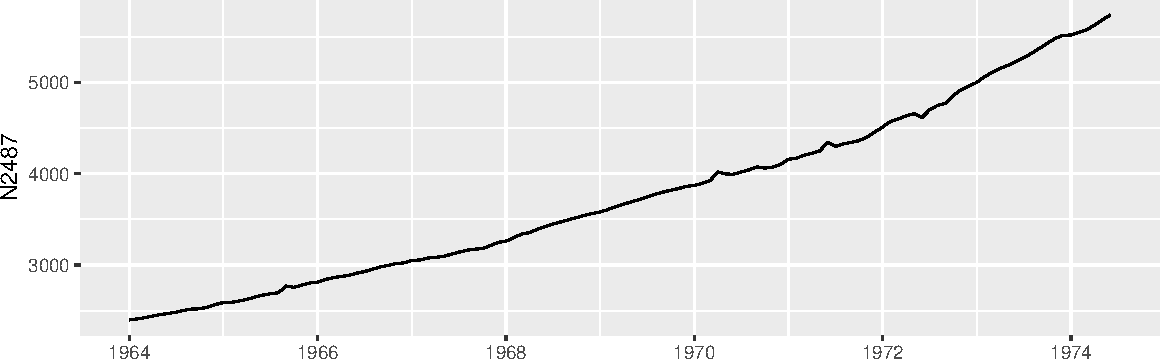
\includegraphics[width=6cm]{M3specLo.pdf}
  \end{block}
\end{textblock}
}
\only<3>{
\begin{textblock}{6}(6.6,3)
  \begin{block}{High Spectral Entropy}
    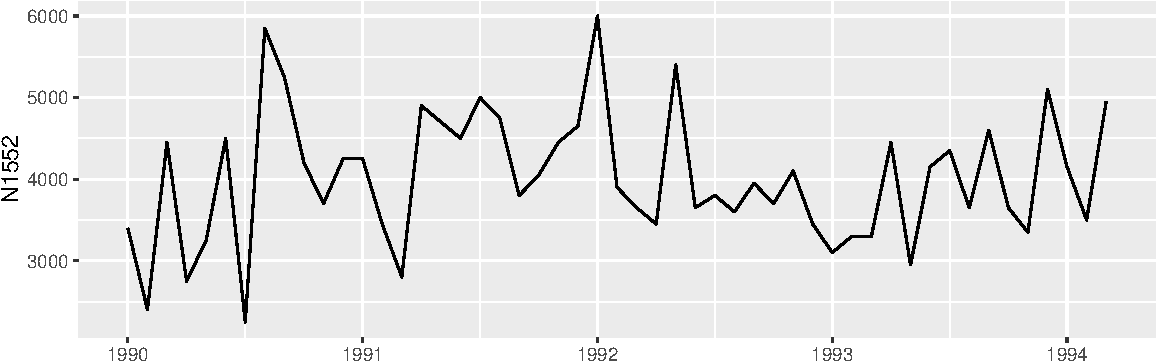
\includegraphics[width=6cm]{M3specHi.pdf}
  \end{block}
\end{textblock}
}\end{frame}

% \begin{frame}{Distribution of Box-Cox for M3}
% \fullwidth{kdeLambda}
% \only<2->{
% \begin{textblock}{6}(0.2,3)
%   \begin{block}{Low Box-Cox}
%     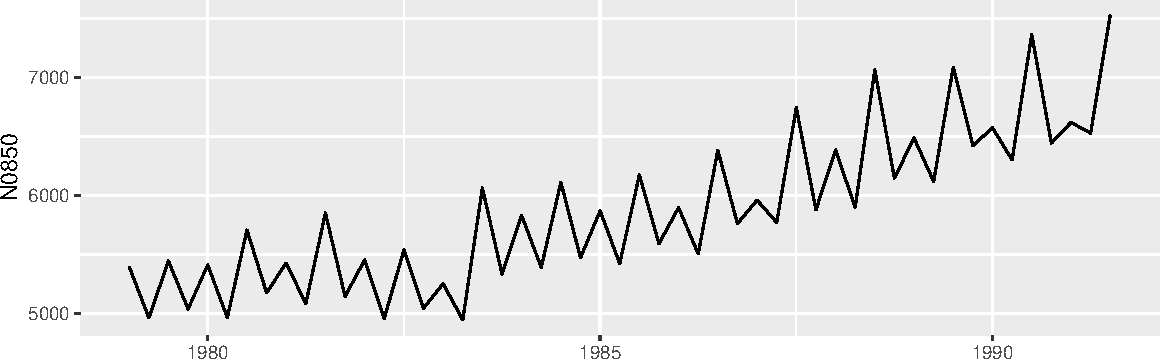
\includegraphics[width=6cm]{M3lambdaLo.pdf}
%   \end{block}
% \end{textblock}
% }
% \only<3>{
% \begin{textblock}{6}(6.6,3)
%   \begin{block}{High Box-Cox}
%     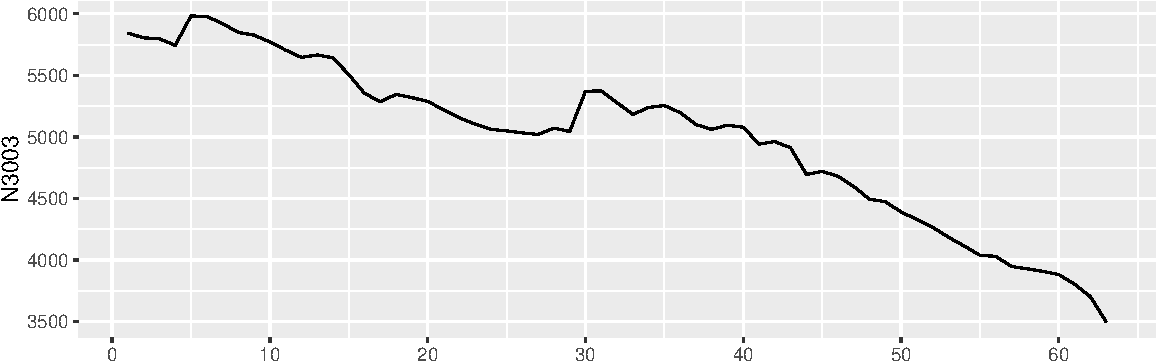
\includegraphics[width=6cm]{M3lambdaHi.pdf}
%   \end{block}
% \end{textblock}
% }
% \end{frame}

\begin{frame}{Feature distributions}
\fullwidth{ACF1SE}
\end{frame}


\begin{frame}{Feature distributions}
\fullwidth{TrendSE}
\end{frame}

\begin{frame}{Feature distributions}
\placefig{2}{1.5}{height=8.2cm,width=8.4cm}{PairwisePlot}
\end{frame}

\begin{frame}{\large Dimension reduction for time series}

\only<1->{\placefig{0}{1.3}{width=4cm,height=8.3cm,trim=0 0 200 0,clip=TRUE}{M3sample}}
\only<2->{\placefig{6}{1.3}{width=4.5cm}{PairwisePlot}}
\only<3>{\placefig{5.5}{6.3}{width=5.5cm}{InstanceSpace}}

\only<2->{\placefig{4}{2.3}{width=2cm}{arrow}}
\only<3>{\placefig{8.4}{4.8}{width=2cm,angle=-90}{arrow}}

\only<2->{\begin{textblock}{2.1}(4,2.9)
\begin{alertblock}{}\small
Feature calculation
\end{alertblock}
\end{textblock}}

\only<3->{\begin{textblock}{2.8}(9.7,4.4)
\begin{alertblock}{}\small
Principal component decomposition
\end{alertblock}
\end{textblock}}

\end{frame}

\begin{frame}{Feature space of M3 data}
\only<1>{\placefig{0.2}{1.2}{height=8cm,width=11.13cm}{InstanceSpace}}
\only<2>{\placefig{0.2}{1.2}{height=8cm,width=12.28cm}{Feature4}}
\only<3>{\placefig{0.2}{1.2}{height=8cm,width=12.35cm}{Feature1}}
\only<4>{\placefig{0.2}{1.2}{height=8cm,width=12.5cm}{Feature2}}
\only<5>{\placefig{0.2}{1.2}{height=8cm,width=12.5cm}{Feature3}}
\only<6>{\placefig{0.2}{1.2}{height=8cm,width=12.5cm}{Feature5}}
%\only<7>{\placefig{0.2}{1.2}{height=8cm,width=12.5cm}{Feature6}}

\end{frame}

\begin{frame}{What about the holes?}
\placefig{0.2}{1.2}{height=8cm,width=11.13cm}{InstanceSpace}
\only<2->{\begin{textblock}{3}(1.2,1.8)\alert{What time series live here?}\end{textblock}}
\only<3->{\begin{textblock}{4}(8.2,7.8)\alert{Or here?}\end{textblock}}
\only<4>{\begin{textblock}{4}(8.7,1.8)\alert{Or here?}\end{textblock}}


\end{frame}

\begin{frame}{Generating new time series}\fontsize{13}{14.5}\sf

\begin{block}{}
We can use the feature space to:
\begin{itemize}
\item[\ding{229}] Generate new time series with similar features to existing series
\item[\ding{229}] Generate new time series where there are ``holes'' in the feature space.
\end{itemize}
\end{block}
\pause\vspace*{-0.4cm}

\begin{itemize}
\item Let $\{\text{PC}_1,\text{PC}_2,\dots,\text{PC}_{n}\}$ be a ``population'' of time series of specified length and period.
\item Genetic algorithm uses a process of selection, crossover and mutation to evolve the population towards a target point $T_i$.
\item Optimize: $\text{Fitness }(\text{PC}_j) = - \sqrt{(|\text{PC}_j-T_i|^2)}$.
\item Initial population random with some series in neighbourhood of $T_i$.
\end{itemize}
\end{frame}

\begin{frame}{Evolving new time series}
\only<1>{\fullheight{TargetedInstancesEgsLocations} }
\only<2>{\fullheight{EvolvedInstancesEgs} }

\end{frame}
\begin{frame}{Evolving new time series}
\only<1>{\fullheight{UnknownEvolvedEgsLocations}}
\only<2>{\fullheight{UnknownEvolvedEgs}}
\end{frame}

\begin{frame}{Evolving new time series}
\only<1>{\placefig{2.1}{1.4}{height=7.6cm, trim=30 600 550 0, clip=TRUE}{EvolvedTSnbDiffLsep}}
\only<2>{\placefig{2.1}{1.4}{height=7.6cm, trim=606 600 0 0, clip=TRUE}{EvolvedTSnbDiffLsep}}
\only<3>{\placefig{2.1}{1.4}{height=7.52cm, trim=30 30 570 577, clip=TRUE}{EvolvedTSnbDiffLsep}}
\only<4>{\placefig{2.1}{1.4}{height=7.52cm, trim=606 30 0 577, clip=TRUE}{EvolvedTSnbDiffLsep}}
\begin{textblock}{3}(6,9)PC1\end{textblock}
\begin{textblock}{3}(1.3,4.55)PC2\end{textblock}

\end{frame}

\begin{frame}{Papers and packages}

\hspace*{-0.4cm}\begin{tabular}{lp{8.5cm}}
\raisebox{-2.3cm}{
\includegraphics[width=2cm]{IJFcover.jpg}} & \RaggedRight Kang, Hyndman, \& Smith-Miles, K. (2017) Visualising forecasting algorithm performance using time series instance spaces. \emph{IJF}, \textbf{33}(2) 345--358. \\[0.6cm]
\raisebox{-1.5cm}{
\includegraphics[width=2cm]{Rlogo}} & \RaggedRight Hyndman, Wang, Kang, Talagala \& Montero-Manso (2018). \textbf{tsfeatures}: Time Series Feature Extraction. \par
  \rlap{\url{github.com/robjhyndman/tsfeatures/}}
\end{tabular}

\end{frame}


%\section{Comparing forecasting methods}

% \begin{frame}{Predictability}
% \begin{block}{Six forecasting methods:}
% \begin{enumerate}
% \item \textbf{Na\"{i}ve}%: Last observed value
% \item \textbf{Seasonal Na\"{i}ve}%: Last observed value from each season
% \item \textbf{Theta method}%: No seasonal adjustment applied
% \item \textbf{ETS}%: Implemented in \texttt{ets()} in R.
% \item \textbf{autoARIMA}%: Implemented in \texttt{auto.arima()} in R.
% \item \textbf{STL-AR}%:  Implemented in \texttt{stlf()} in R.
% \end{enumerate}
% \end{block}\pause
% \begin{alertblock}{}
% Compute minimum MASE from all methods
% \end{alertblock}
% \end{frame}


% \begin{frame}{Predictability: MASE values}
% \only<1>{\placefig{0.2}{1.2}{height=8cm,width=11.32cm}{MASElo}}
% \only<2>{\placefig{0.2}{1.2}{height=8cm,width=11.32cm}{MASEmid}}
% \only<3>{\placefig{0.2}{1.2}{height=8cm,width=11.32cm}{MASEhi}}
% \end{frame}


% \begin{frame}{Predictability: Comparing methods}
% \only<1>{\placefig{0.2}{1.2}{height=8cm}{MASE1}}
% \only<2>{\placefig{0.2}{1.2}{height=8cm}{MASE2}}
% \only<3>{\placefig{0.2}{1.2}{height=8cm}{MASE3}}
% \only<4>{\placefig{0.2}{1.2}{height=8cm}{MASE4}}
% \only<5>{\placefig{0.2}{1.2}{height=8cm}{MASE5}}
% \only<6>{\placefig{0.2}{1.2}{height=8cm}{MASE6}}
% \end{frame}

% \begin{frame}{Predictability}
% \only<1>{\placefig{1}{1}{height=8cm}{snaive}}
% \only<2>{\placefig{1}{1}{height=8cm}{arima}}
% \end{frame}

% \begin{frame}{MASE values}

% \only<1>{\begin{block}{MASE values on M3 data}\centering
% \begin{tabular}{llllllll}
%   Method              & Yearly   & Quarterly & Monthly  & All  \\
%   \midrule
%   Na\"{\i}ve          & 3.17     & 1.46      & 1.17     & 1.79 \\
%   Seasonal na\"{\i}ve & 3.17     & 1.43      & 1.15     & 1.76 \\
%   Theta               & \bf 2.77 & 1.30      & 1.02     & 1.54 \\
%   ETS                 & 2.86     & \bf 1.18  & \bf 0.86 & \bf 1.43 \\
%   ARIMA               & 2.96     & 1.19      & 0.88     & 1.46 \\
%   STL-AR              & 2.95     & 1.91      & 1.27     & 1.83 \\
% \end{tabular}
% \end{block}}

% \only<2>{\begin{block}{MASE values on evolved data}\centering
% \begin{tabular}{llllllll}
%   Method              & Yearly   & Quarterly & Monthly  & All  \\
%   \midrule
%   Na\"{\i}ve          & \bf 1.93 & 3.10      & 2.35     & 2.46 \\
%   Seasonal na\"{\i}ve & 1.93     & 1.40      & 1.21     & \bf 1.51 \\
%   Theta               & 2.09     & 3.02      & 2.17     & 2.43 \\
%   ETS                 & 2.67     & \bf 1.07  & \bf 0.93 & 1.56 \\
%   ARIMA               & 2.46     & 1.13      & 0.94     & \bf 1.51 \\
%   STL-AR              & 2.44     & 1.35      & 1.08     & 1.62 \\
% \end{tabular}
% \end{block}}
%\end{frame}


% \begin{frame}{What next?}\vspace*{-0.2cm}
%   \begin{itemize}
%    \item Method allows us to analyse a large collection of time series -- spot unusual time series, clusters of time series, etc.
%    \item These features are not differentiating forecasting methods.
%    \item Generate new time series with controllable characteristics. E.g., more data similar to an existing data set, or data unlike any seen before.
%    \item With better features, we could develop meta-forecasting algorithms which choose a specific forecasting method based on the location of a time series in the feature space.
%   \end{itemize}

% \vspace*{10cm}

% \end{frame}



\section{Finding weird time series}

\begin{frame}{Yahoo web-traffic}\vspace*{-0.2cm}\fontsize{13}{15}\sf
  \begin{itemize}
    \item Tens of thousands of time series collected at one-hour intervals over one month.
    \item Consisting of several server metrics (e.g. CPU usage and paging views)
      from many server farms globally.
\item Aim: find unusual (anomalous) time series.
  \end{itemize}\vspace*{10cm}
\placefig{0}{4.6}{width=13.7cm, trim=0 20 0 220, clip=TRUE}{serverfarm}
\end{frame}

\begin{frame}{Yahoo web-traffic}
\centerline{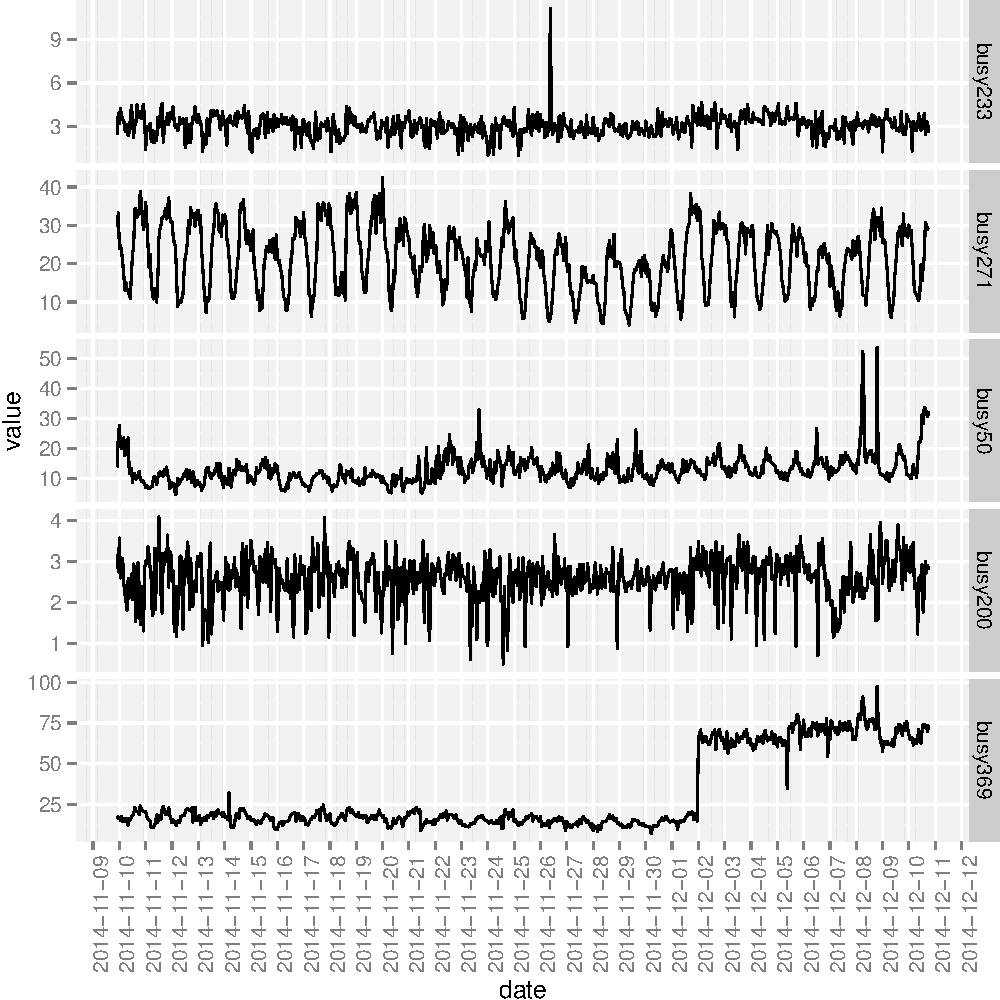
\includegraphics[width=4.3cm, clip=true, trim=30 10 20 0, height=8cm]{busy_eg.pdf}
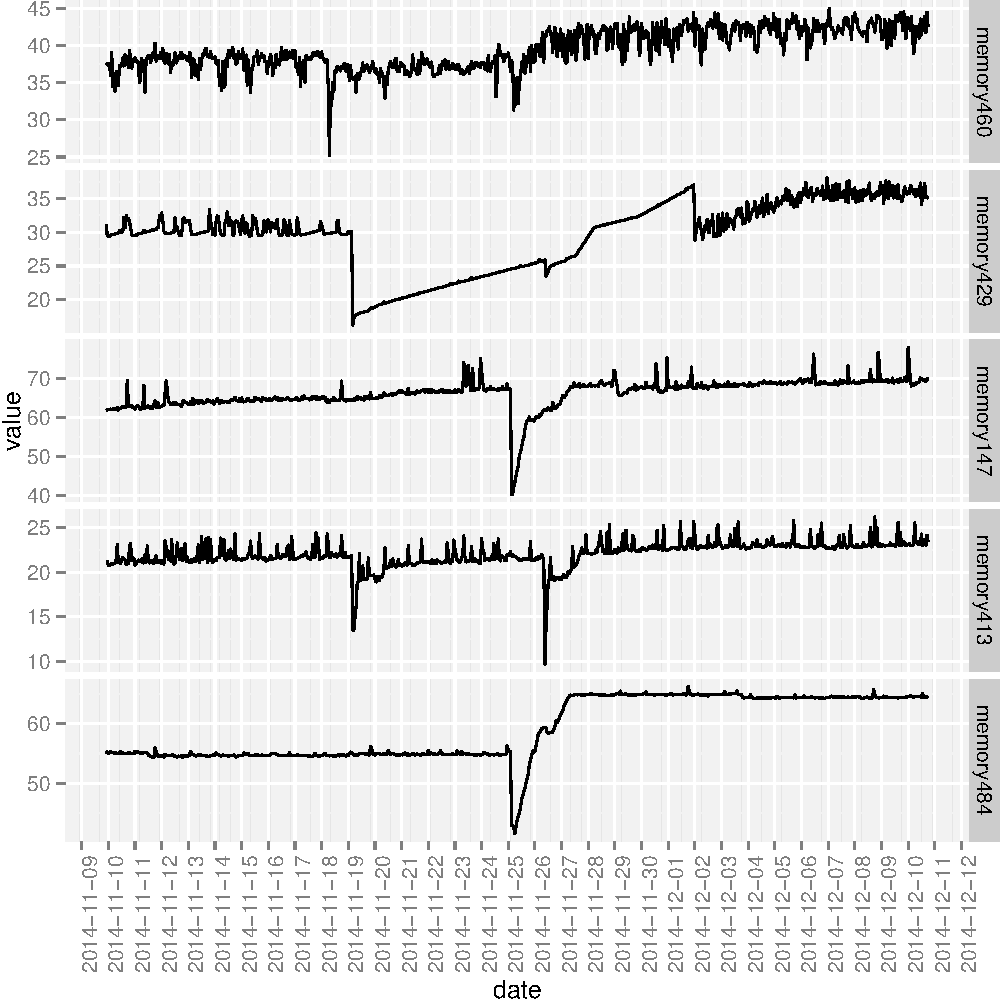
\includegraphics[width=4.3cm, clip=true, trim=30 10 20 0, height=8cm]{memory_eg.pdf}
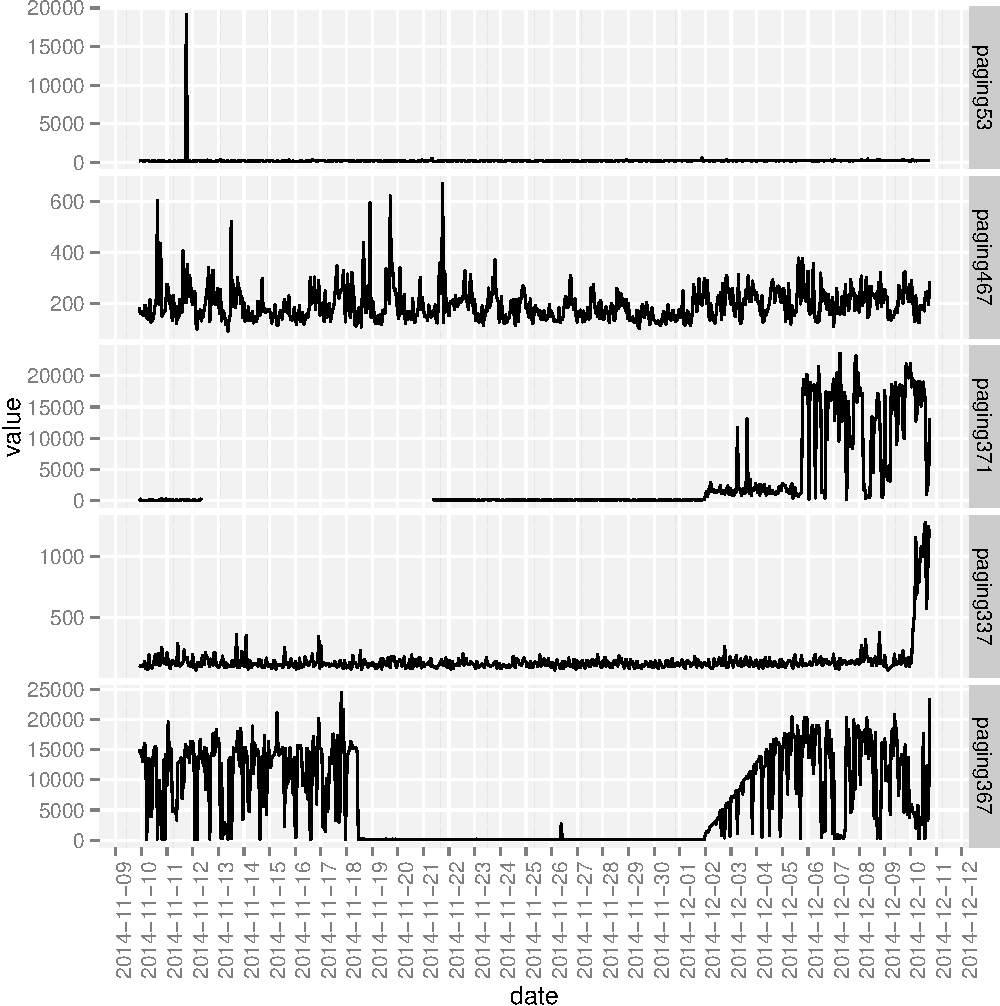
\includegraphics[width=4.3cm, clip=true, trim=30 10 20 0, height=8cm]{page_eg.pdf}}
\end{frame}

\begin{frame}{Feature space}\fontsize{10}{11}\sf\vspace*{-0.2cm}
\begin{itemize}
\item \textbf{ACF1}: first order autocorrelation = $\text{Corr}(Y_t,Y_{t-1})$
\item Strength of \textbf{trend} and \textbf{seasonality} based on STL
\item Trend \textbf{linearity} and \textbf{curvature}
\item Size of seasonal \textbf{peak} and \textbf{trough}
\item Spectral \textbf{entropy}
\item \textbf{Lumpiness}: variance of block variances (block size 24).
\item \textbf{Spikiness}: variances of leave-one-out variances of STL remainders.
\item \textbf{Level shift}: Maximum difference in trimmed means of consecutive moving windows of size 24.
\item \textbf{Variance change}: Max difference in variances of consecutive moving windows of size 24.
\item \textbf{Flat spots}: Discretize sample space into 10 equal-sized intervals. Find max run length in any interval.
\item Number of \textbf{crossing points} of mean line.
 \item \textbf{Kullback-Leibler score}:
      Maximum of $        D_{KL}(P\|Q) = \int P(x)\ln P(x)/ Q(x) dx$
       where $P$ and $Q$ are estimated by kernel density estimators applied to
       consecutive windows of size 48.
\item \textbf{Change index}: Time of maximum KL score
\end{itemize}
\end{frame}

\begin{frame}{Principal component analysis}
\centerline{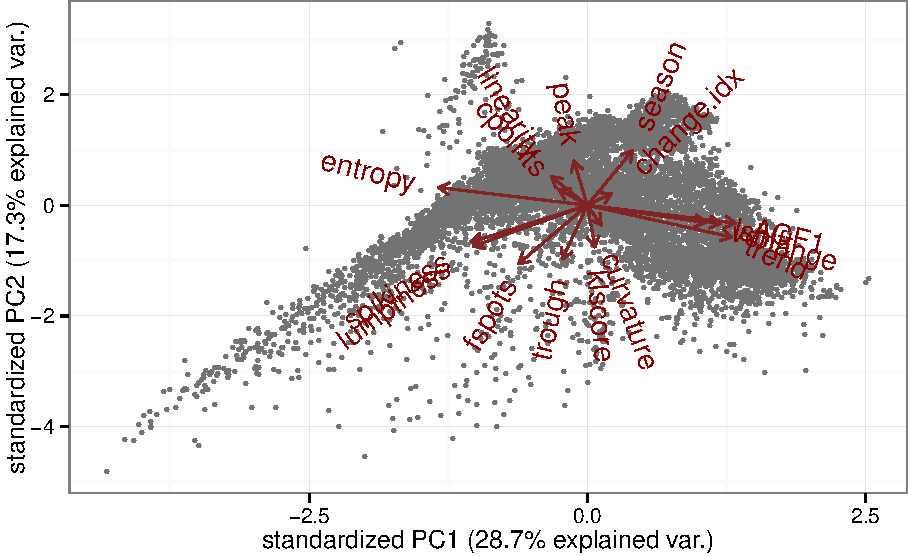
\includegraphics[width=12.5cm]{pca}}
\end{frame}


\begin{frame}{What is ``anomalous''?}\fontsize{13}{15}\sf
\centerline{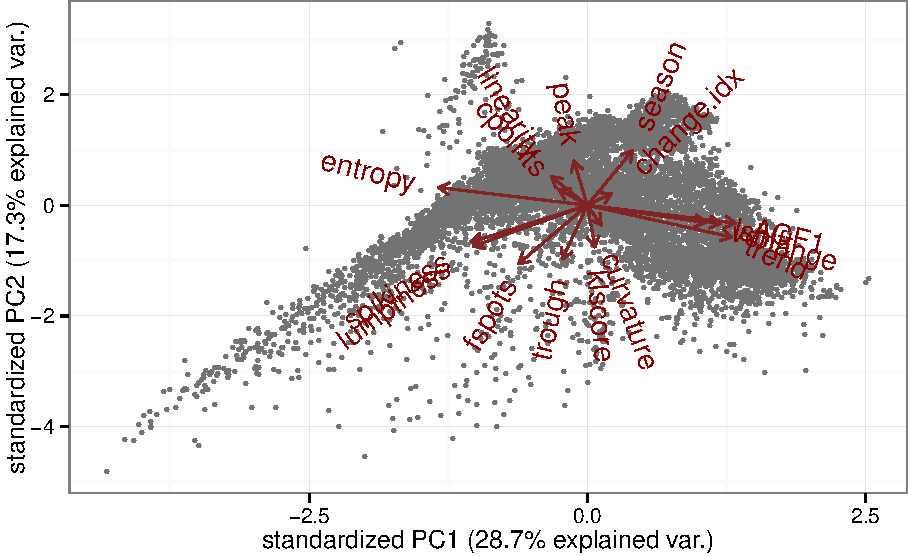
\includegraphics[width=8.5cm]{pca}}
We need a measure of the ``anomalousness'' of a time series.
\pause

Idea: We rank points based on their local density using a bivariate kernel density estimate.

\end{frame}


\begin{frame}{Bivariate kernel density}
\begin{block}{}
  \begin{equation*}
    \hat{f}(\x; \H) = \frac{1}{n}\sum_{i=1}^n K_{\H}(\x - \X_i)
  \end{equation*}
\end{block}\pause
\begin{itemize}
  \item $\X_i \in$ a bivariate random sample $\{\X_1, \X_2, \ldots, \X_n\}$
  \item $K_{\H}(\x)$ is the standard normal kernel function
  % \item $\H = diag(h_1^2, h_2^2)$ parallel to the co-ordinate axes
  \item $\H$ estimated by minimizing the sum of AMISE
  \item Rank points based on $\hat{f}$ values in 2d PCA space.
\end{itemize}
\end{frame}


\begin{frame}{Bivariate density ranking}
\only<1>{\fullwidth{yahoohdr}}
\only<2>{\fullwidth{hdrout}}
\end{frame}



% %\section{What next?}

% \begin{frame}{What next?}\fontsize{14}{15}\sf
%   \begin{itemize}
%     \item Develop a more comprehensive set of features that are reliable measures and fast to compute. e.g., for finance data.
%     \item Consider other dimension reduction methods and more than 2 dimensions.
%     \item Develop dynamic and interactive visualization tools.
%     \item Some of the methods are already available in the \textbf{anomalous} package for R on github.
%     \item Currently working on a more general time series features package.
%   \end{itemize}
% \end{frame}

\begin{frame}{Security monitoring}

\placefig{0}{1.2}{width=13cm, height=6cm}{1_climb}

\end{frame}

\begin{frame}{Security monitoring}

\placefig{0}{1.2}{width=13cm, height=6cm}{1_climb}

\vspace*{4.2cm}

\hspace*{5.3cm}

\animategraphics[loop,autoplay,controls=false,height=3.9cm]{12}{figs/streaming-}{0}{134}

\end{frame}

\begin{frame}{Time series anomaly detection}

\begin{itemize}
\item Density-based outliers vs distance-based outliers.

\item Fast feature calculation using windows needed for streaming data.

\item \textbf{Oddstream}: Density-based anomalies, requiring a ``typical'' training period.
\item \textbf{Stray}: Distance-based anomalies, requiring no ``typical'' training period.
\end{itemize}


\end{frame}


\begin{frame}{Papers and packages}\fontsize{11}{11}\sf

\begin{tabular}{lp{9cm}}
\raisebox{-1.cm}{
\includegraphics[width=1cm]{IJFcover}} & \RaggedRight Hyndman, Wang \& Laptev (2015). Large-scale unusual time series detection. \emph{Proceedings of the IEEE International Conference on Data Mining}.  \\[0.15cm]
\raisebox{-1.3cm}{\fbox{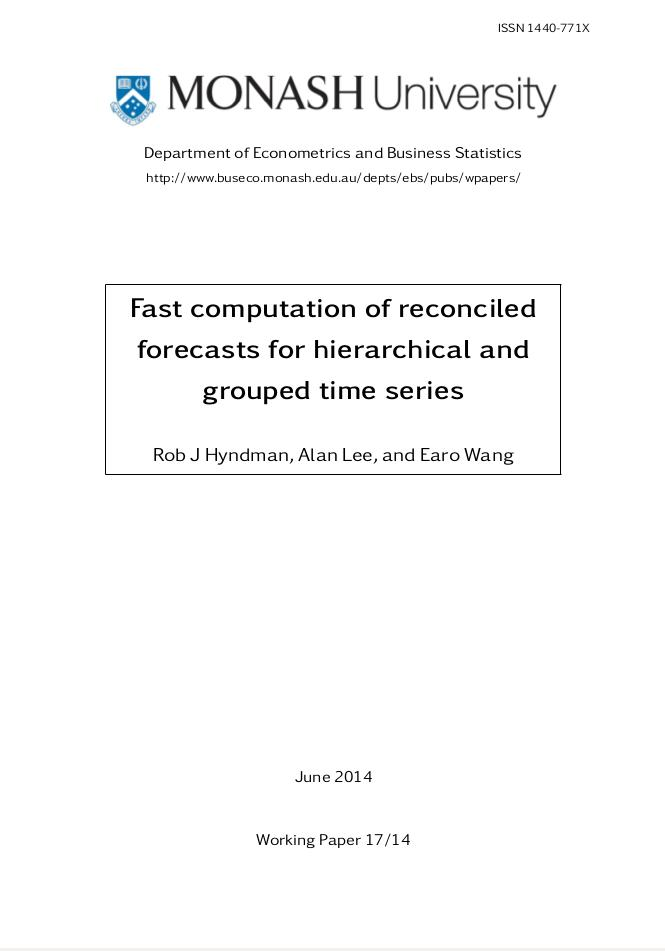
\includegraphics[width=1cm]{wpcover}}} & \RaggedRight Talagala, Hyndman, Smith-Miles, Kandanaarachchi \& Muñoz (2018) Anomaly detection in streaming nonstationary temporal data. 
\par\url{robjhyndman.com/publications/oddstream/}\\[0.15cm]
\raisebox{-.6cm}{
\includegraphics[width=1cm]{Rlogo}} & \RaggedRight Hyndman, Wang, Kang, Talagala \& Montero-Manso (2018). \textbf{tsfeatures}: Time Series Feature Extraction.  \url{github.com/robjhyndman/tsfeatures/}\\[0.15cm]
\raisebox{-.6cm}{
\includegraphics[width=1cm]{Rlogo}} & \RaggedRight Talagala, Hyndman \& Smith-Miles (2018) \textbf{oddstream}: Outlier Detection in Data Streams.  \par\url{github.com/pridiltal/oddstream/}\\[0.15cm]
\raisebox{-.6cm}{
\includegraphics[width=1cm]{Rlogo}} & \RaggedRight Hyndman, Wang, Kang, Talagala \& Montero-Manso (2018). \textbf{stray}: Robust Anomaly Detection in Data Streams with Concept Drift. \url{github.com/pridiltal/stray/}

\end{tabular}


\end{frame}




\section{Reconciling many forecasts}

\begin{frame}{Forecast reconciliation}

\begin{textblock}{12.4}(0.2,1.4)
\begin{block}{}\fontsize{2}{2}\sf
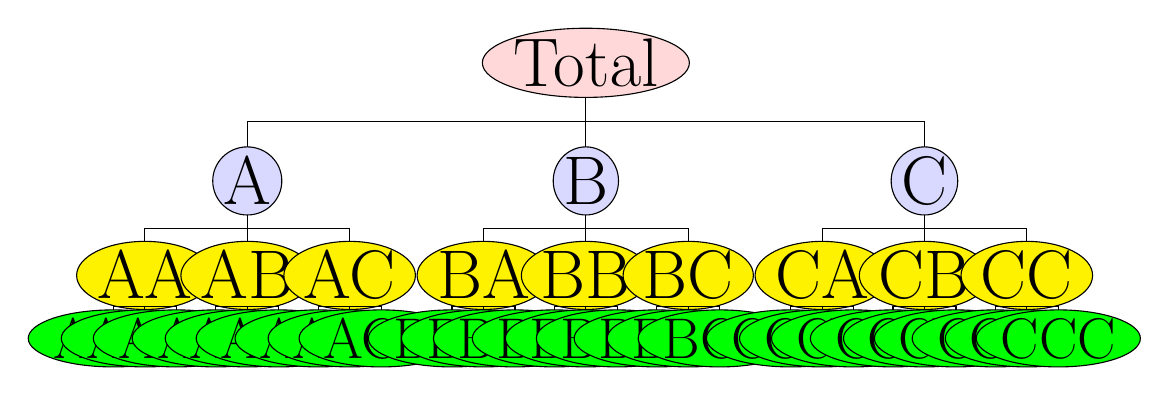
\begin{tikzpicture}
\tikzstyle{every node}=[ellipse,draw,inner sep=0.2pt,outer sep=0pt]
\tikzstyle{level 1}=[sibling distance=43mm,fontscale=14,set style={{every node}+=[fill=blue!15]},level distance=1.5cm]
\tikzstyle{level 2}=[sibling distance=13mm,fontscale=8,set style={{every node}+=[fill=yellow]}, level distance=1.2cm]
\tikzstyle{level 3}=[sibling distance=4mm,fontscale=4,set style={{every node}+=[fill=green]}, level distance=0.8cm]
\node[fill=red!15,fontscale=16]{Total}[edge from parent fork down]
 child {node {A}
   child {node {AA}
     child {node {AAA}}
     child {node {AAB}}
     child {node {AAC}}}
   child {node {AB}
     child {node {ABA}}
     child {node {ABB}}
     child {node {ABC}}}
   child {node {AC}
      child {node {ACA}}
     child {node {ACB}}
     child {node {ACC}}}
 }
 child {node {B}
   child {node {BA}
     child {node {BAA}}
     child {node {BAB}}
     child {node {BAC}}}
   child {node {BB}
     child {node {BBA}}
     child {node {BBB}}
     child {node {BBC}}}
   child {node {BC}
      child {node {BCA}}
     child {node {BCB}}
     child {node {BCC}}}
 }
 child {node {C}
   child {node {CA}
     child {node {CAA}}
     child {node {CAB}}
     child {node {CAC}}}
   child {node {CB}
     child {node {CBA}}
     child {node {CBB}}
     child {node {CBC}}}
   child {node {CC}
      child {node {CCA}}
     child {node {CCB}}
     child {node {CCC}}}
 };
\end{tikzpicture}
\end{block}
\end{textblock}

\vspace*{5.5cm}\fontsize{14}{16}\sf

\begin{itemize}
\item Walmart sales by division, group, sub-group, etc.
\item Australian tourism demand by state, region, zone.
\end{itemize}

\end{frame}

\begin{frame}{Australian tourism demand}
\fullheight{regions1_with_labels}
\only<2>{\begin{textblock}{9}(.5,1.2)\small
\begin{block}{}
  \begin{itemize}\itemsep=0cm\parskip=0cm
    \item Quarterly data on visitor night from 1998:Q1 -- 2013:Q4
    \item From \textit{National Visitor Survey}, based on annual interviews of 120,000 Australians aged 15+, collected by Tourism Research Australia.
    \item Split by 7 states, 27 zones and 76 regions (a~geographical hierarchy)
    \item Also split by purpose of travel
      \begin{itemize}
        \item Holiday
        \item Visiting friends and relatives (VFR)
        \item Business
        \item Other
      \end{itemize}
    \item 304 bottom-level series
  \end{itemize}
\end{block}
\end{textblock}}


\end{frame}




\begin{frame}{Hierarchical time series}

\begin{minipage}{4cm}\vspace*{0.2cm}
\begin{block}{}\centering
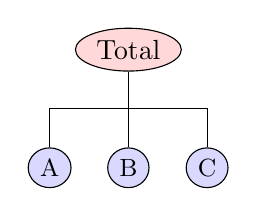
\begin{tikzpicture}
\tikzstyle{every node}=[ellipse,draw,fill=red!15,inner sep=2pt]
\tikzstyle[level distance=.3cm]
\tikzstyle[sibling distance=12cm]
\tikzstyle{level 1}=[sibling distance=10mm,font=\small,set style={{every node}+=[fill=blue!15]}]
\node{Total}[edge from parent fork down]
 child {node {A}
 }
 child {node {B}
 }
 child {node {C}
 };
\end{tikzpicture}
\end{block}
\end{minipage}
{\small
\only<2->{\begin{textblock}{6.3}(6,1)
\begin{itemize}\itemsep=0cm\parskip=0cm
\item[ $ y_{t}: $] observed aggregate of all series at time
$t$.
\item[ $ y_{X,t}: $] observation on series $X$ at time $t$.
\item[ $ \bm{b}_{t}: $] vector of all series at bottom level
in time $t$.
\end{itemize}
\end{textblock}}}\vspace*{0.6cm}
\only<3->{
$\by_{t}= [y_{t},y_{A,t},y_{B,t},y_{C,t}]' = \only<3>{\hspace*{-0.08cm}\begin{pmatrix}
                1 & 1 & 1 \\
                1 & 0 & 0 \\
                0 & 1 & 0\\
                0 & 0 & 1
                \end{pmatrix}}\only<4->{{\color{red}\underbrace{\begin{pmatrix}
                1 & 1 & 1 \\
                1 & 0 & 0 \\
                0 & 1 & 0\\
                0 & 0 & 1
                \end{pmatrix}}_{\bS}}}\only<4>{\hspace*{0.08cm}}\only<3-4>{\hspace*{-0.1cm}\begin{pmatrix}y_{A,t}\\y_{B,t}\\y_{C,t}\end{pmatrix}}\rule{0cm}{1.6cm}
                \only<5->{\hspace*{0.08cm}{\color{blue}\underbrace{\begin{pmatrix}y_{A,t}\\y_{B,t}\\y_{C,t}\end{pmatrix}}_{\bm{b}_{t}}}}$}


\vspace*{-0.6cm}

\only<6>{\colorbox[gray]{.8}{$\by_{t}=\color{red}\bS\color{blue}\bm{b}_{t}$}}

\vspace*{10cm}

\end{frame}

% \begin{frame}{Hierarchical time series}\vspace*{-0.3cm}


% \begin{block}{}\hspace*{.6cm}{\centering\small
% \begin{tikzpicture}[level distance=1cm]
% \tikzstyle{every node}=[ellipse,draw,fill=red!15,inner sep=2pt]
% \tikzstyle[level distance=.01cm]
% \tikzstyle[sibling distance=12cm]
% \tikzstyle{level 2}=[sibling distance=10mm,font=\scriptsize,set style={{every node}+=[fill=yellow]}]
% \tikzstyle{level 1}=[sibling distance=40mm,font=\footnotesize,set style={{every node}+=[fill=blue!15]}]
% \node{Total}[edge from parent fork down]
%  child {node {A}
%    child {node {AX}}
%    child {node {AY}}
%    child {node {AZ}}
%  }
%  child {node {B}
%    child {node {BX}}
%    child {node {BY}}
%    child {node {BZ}}
%  }
%  child {node {C}
%    child {node {CX}}
%    child {node {CY}}
%    child {node {CZ}}
%  };
% \end{tikzpicture}}
% \end{block}\vspace*{0.1cm}\pause\fontsize{13}{15}\sf

% \hbox{$\by_{t}= {\scriptsize\begin{pmatrix}
%     y_t\\
%     y_{A,t}\\
%     y_{B,t}\\
%     y_{C,t}\\
%     y_{AX,t}\\
%     y_{AY,t}\\
%     y_{AZ,t}\\
%     y_{BX,t}\\
%     y_{BY,t}\\
%     y_{BZ,t}\\
%     y_{CX,t}\\
%     y_{CY,t}\\
%     y_{CZ,t}\end{pmatrix}}=
%     {\color{red}\underbrace{\scriptsize\begin{pmatrix}
%                 1 & 1 & 1 & 1 & 1 & 1 & 1 & 1 & 1\\
%                 1 & 1 & 1 & 0 & 0 & 0 & 0 & 0 & 0\\
%                 0 & 0 & 0 & 1 & 1 & 1 & 0 & 0 & 0\\
%                 0 & 0 & 0 & 0 & 0 & 0 & 1 & 1 & 1\\
%                 1 & 0 & 0 & 0 & 0 & 0 & 0 & 0 & 0\\
%                 0 & 1 & 0 & 0 & 0 & 0 & 0 & 0 & 0\\
%                 0 & 0 & 1 & 0 & 0 & 0 & 0 & 0 & 0\\
%                 0 & 0 & 0 & 1 & 0 & 0 & 0 & 0 & 0\\
%                 0 & 0 & 0 & 0 & 1 & 0 & 0 & 0 & 0\\
%                 0 & 0 & 0 & 0 & 0 & 1 & 0 & 0 & 0\\
%                 0 & 0 & 0 & 0 & 0 & 0 & 1 & 0 & 0\\
%                 0 & 0 & 0 & 0 & 0 & 0 & 0 & 1 & 0\\
%                 0 & 0 & 0 & 0 & 0 & 0 & 0 & 0 & 1\\
%              \end{pmatrix}}_{\bS}}{\color{blue}\underbrace{\scriptsize\begin{pmatrix}
%     y_{AX,t}\\
%     y_{AY,t}\\
%     y_{AZ,t}\\
%     y_{BX,t}\\
%     y_{BY,t}\\
%     y_{BZ,t}\\
%     y_{CX,t}\\
%     y_{CY,t}\\
%     y_{CZ,t}\end{pmatrix}}_{\bm{b}_{t}}}$}

%     \vspace*{10cm}

% \only<3>{\begin{textblock}{3}(10.5,8)\colorbox[gray]{.8}{$\by_{t}=\color{red}\bS\color{blue}\bm{b}_{t}$}\end{textblock}}

% \end{frame}



% \begin{frame}{Grouped data}\vspace*{-0.4cm}


% \begin{block}{}
% \begin{center}\small
% \tikzstyle{every node}=[inner sep=2pt]
% \begin{tikzpicture}
%     \matrix[ampersand replacement=\&,column sep=0.3cm] {
%         \node[ellipse,draw,fill=yellow,font=\scriptsize,distance=1cm] {AX};~ \&
%         \node[ellipse,draw,fill=yellow,font=\scriptsize] {AY};~ \&
%         \node[ellipse,draw,fill=blue!15] {A}; \\[0.3cm]
%         \node[ellipse,draw,fill=yellow,font=\scriptsize] {BX};~ \&
%         \node[ellipse,draw,fill=yellow,font=\scriptsize] {BY};~ \&
%         \node[ellipse,draw,fill=blue!15] {B}; \\[0.3cm]
%         \node[ellipse,draw,fill=blue!15] {X};~ \&
%         \node[ellipse,draw,fill=blue!15] {Y};~ \&
%         \node[ellipse,draw,fill=red!15] {Total}; \\
% };
% \end{tikzpicture}
% \end{center}
% \end{block}\vspace*{0.0cm}\pause\fontsize{13}{14}\sf


% \hbox{$\by_{t}= {\small\begin{pmatrix}
%     y_t\\
%     y_{A,t}\\
%     y_{B,t}\\
%     y_{X,t}\\
%     y_{Y,t}\\
%     y_{AX,t}\\
%     y_{AY,t}\\
%     y_{BX,t}\\
%     y_{BY,t}
%     \end{pmatrix}}=
%     \color{red}\underbrace{\small\begin{pmatrix}
%                 1 & 1 & 1 & 1 \\
%                 1 & 1 & 0 & 0 \\
%                 0 & 0 & 1 & 1 \\
%                 1 & 0 & 1 & 0 \\
%                 0 & 1 & 0 & 1 \\
%                 1 & 0 & 0 & 0 \\
%                 0 & 1 & 0 & 0 \\
%                 0 & 0 & 1 & 0 \\
%                 0 & 0 & 0 & 1
%              \end{pmatrix}}_{\bS} \color{blue}\underbrace{\small\begin{pmatrix}
%     y_{AX,t}\\
%     y_{AY,t}\\
%     y_{BX,t}\\
%     y_{BY,t}
%     \end{pmatrix}}_{\bm{b}_{t}}$}

% \vspace*{-1cm}


% \only<3>{\begin{textblock}{3}(10.5,8)\colorbox[gray]{.8}{$\by_{t}=\color{red}\bS\color{blue}\bm{b}_{t}$}\end{textblock}}

%     \vspace*{10cm}

% \end{frame}


\begin{frame}{\large Disaggregated time series}

Every collection of time series with aggregation constraints can be written as
\begin{block}{}
\centerline{$\by_{t}=\bS\bm{b}_{t}$}
\end{block}
where
\begin{itemize}
\item $\by_t$ is a vector of all series at time $t$
\item $\bm{b}_t$ is a vector of the most disaggregated series at time $t$
\item $\bS$ is a ``summing matrix'' containing the aggregation constraints.
\end{itemize}

\end{frame}




\begin{frame}{Forecasting notation}


Let $\hat{\by}_n(h)$ be vector of initial $h$-step forecasts, made at time $n$, stacked in same order as $\by_t$. \pause\\  (In general, they will not ``add up''.)\pause

\begin{block}{}
Reconciled forecasts must be of the form:

\centerline{$ \tilde{\by}_{n}(h)=\bS\bm{P}\hat{\by}_{n}(h)$}

for some matrix $\bm{P}$.
\end{block}\pause
\biz
\item
$\bm{P}$ maps base forecasts $\hat{\by}_{n}(h)$ to bottom level.
\item
$\bS$ adds them up
\eiz
\end{frame}

\begin{frame}{General properties: bias and variance}

\begin{block}{}
\centerline{$ \tilde{\by}_{n}(h)=\bS\bm{P}\hat{\by}_{n}(h)$}
\end{block}\pause%\fontsize{14}{16.5}\sf

\textbf{\alert{Bias}}
\begin{alertblock}{}\centering
Reconciled forecasts are unbiased iff $\bS\bm{P}\bS=\bS$.\rlap{\phantom{g}}
\end{alertblock}\pause

\textbf{\alert{Variance}}\\
Let error variance of $h$-step base forecasts $\hat{\by}_n(h)$ be
$$\bSigma_h = \var[\by_{n+h} - \hat{\by}_{n}(h) \mid \by_1,\dots,\by_n] $$
Then error variance of the reconciled forecasts is
\begin{alertblock}{}
\centerline{$\var[\by_{n+h} - \tilde{\by}_{n}(h)  \mid \by_1,\dots,\by_n]  = \bS\bm{P}\bSigma_{h}\bm{P}'\bS'$}
\end{alertblock}

%This is a general result for all existing methods.


\end{frame}

\begin{frame}{Optimal forecast reconciliation}
\begin{block}{}
\centerline{$ \tilde{\by}_{n}(h)=\bS\bm{P}\hat{\by}_{n}(h)$}
\end{block}\pause\vspace*{0.4cm}

\begin{alertblock}{Theorem: MinT Reconciliation}
If $\bm{P}$ satisfies $\bm{S}\bm{P}\bm{S} = \bm{S}$,  then

\centerline{$\min_{\bm{P}} = \text{trace}[\bm{S}\bm{P}\bSigma_h\bm{P}'\bm{S}']$}

has solution $\bm{P} = (\bS'\bSigma^{-1}_{h}\bS)^{-1}\bS'\bSigma^{-1}_{h}$.
\end{alertblock}\pause

\only<3->{
\begin{textblock}{8}(2.4,6)
\begin{block}{}
\centerline{$\displaystyle\textcolor{red}{\tilde{\by}_{n}(h)}
=\bS(\bS'\bSigma^{-1}_{h}\bS)^{-1}\bS'\bSigma^{-1}_{h}\textcolor{blue}{\hat{\by}_{n}(h)}$}
\end{block}\end{textblock}}\vspace*{1.3cm}


\hspace*{-0.2cm}\hbox to 11.2cm{\textcolor{red}{Reconciled forecasts}\hfill\textcolor{blue}{Base forecasts}}


\vspace*{10cm}


\end{frame}

\begin{frame}{Optimal forecast reconciliation}


\begin{textblock}{8}(2.4,1.4)
\begin{block}{}
\centerline{$\displaystyle\textcolor{red}{\tilde{\by}_{n}(h)}
=\bS(\bS'\bSigma^{-1}_{h}\bS)^{-1}\bS'\bSigma^{-1}_{h}\textcolor{blue}{\hat{\by}_{n}(h)}$}
\end{block}\end{textblock}\vspace*{1.3cm}

\hspace*{-0.2cm}\hbox to 11.2cm{\textcolor{red}{Reconciled forecasts}\hfill\textcolor{blue}{Base forecasts}}
\pause\vspace*{-0.4cm}

Assume that $\bSigma_h =k_h \bSigma_1$ to simplify computations.

\pause

\begin{block}{WLS solution}
\begin{itemize}
\item Approximate $\bSigma_1$ by its diagonal.
\end{itemize}
\end{block}

\pause

\begin{block}{GLS solution}
\begin{itemize}
\item Estimate $\bSigma_1$ using shrinkage to the diagonal.
\end{itemize}
\end{block}

\vspace*{10cm}

\end{frame}



%\section{Application: Australian tourism}

\begin{frame}{Australian \rlap{tourism}}
\fullheight{regions1_with_labels}
\only<2-3>{\begin{textblock}{6.8}(2,2)
\begin{block}{Hierarchy:}
  \begin{itemize}
    \item States (7)
    \item Zones (27)
    \item Regions (82)
  \end{itemize}
\end{block}
\end{textblock}}
\only<3>{\begin{textblock}{6.8}(2,6)
\begin{block}{Base forecasts}
ETS (exponential smoothing) models
\end{block}\end{textblock}}


\end{frame}

\begin{frame}{Base forecasts}
\only<1>{\fullwidth{austourism1}}
\only<2>{\fullwidth{austourism2}}
\only<3>{\fullwidth{austourism3}}
\only<4>{\fullwidth{austourism4}}
\only<5>{\fullwidth{austourism5}}
\only<6>{\fullwidth{austourism6}}
\only<7>{\fullwidth{austourism7}}
\only<8>{\fullwidth{austourism8}}
\only<9>{\fullwidth{austourism9}}
\end{frame}

% \begin{frame}{Reconciled forecasts}
% \only<1>{\fullwidth{Australia}}
% \only<2>{\fullwidth{States}}
% \only<3>{\fullwidth{Capitals}}
% \end{frame}

\begin{frame}{Forecast evaluation}
\begin{textblock}{14}(0.3,1.5)
\textbf{\textcolor{blue}{Training sets}} \hspace*{3cm}
\textbf{\textcolor{red}{Test sets
\only<1-20>{$h=1$}%
\only<21>{$h=2$}%
\only<22>{$h=3$}%
\only<23>{$h=4$}%
\only<24>{$h=5$}%
\only<25>{$h=6$}%
}}

\end{textblock}
\only<1>{\placefig{0.0}{2.3}{width=12.6cm}{rorigin1}}
\only<2>{\placefig{0.0}{2.3}{width=12.6cm}{rorigin2}}
\only<3>{\placefig{0.0}{2.3}{width=12.6cm}{rorigin3}}
\only<4>{\placefig{0.0}{2.3}{width=12.6cm}{rorigin4}}
\only<5>{\placefig{0.0}{2.3}{width=12.6cm}{rorigin5}}
\only<6>{\placefig{0.0}{2.3}{width=12.6cm}{rorigin6}}
\only<7>{\placefig{0.0}{2.3}{width=12.6cm}{rorigin7}}
\only<8>{\placefig{0.0}{2.3}{width=12.6cm}{rorigin8}}
\only<9>{\placefig{0.0}{2.3}{width=12.6cm}{rorigin9}}
\only<10>{\placefig{0.0}{2.3}{width=12.6cm}{rorigin10}}
\only<11>{\placefig{0.0}{2.3}{width=12.6cm}{rorigin11}}
\only<12>{\placefig{0.0}{2.3}{width=12.6cm}{rorigin12}}
\only<13>{\placefig{0.0}{2.3}{width=12.6cm}{rorigin13}}
\only<14>{\placefig{0.0}{2.3}{width=12.6cm}{rorigin14}}
\only<15>{\placefig{0.0}{2.3}{width=12.6cm}{rorigin15}}
\only<16>{\placefig{0.0}{2.3}{width=12.6cm}{rorigin16}}
\only<17>{\placefig{0.0}{2.3}{width=12.6cm}{rorigin17}}
\only<18>{\placefig{0.0}{2.3}{width=12.6cm}{rorigin18}}
\only<19>{\placefig{0.0}{2.3}{width=12.6cm}{rorigin19}}
\only<20>{\placefig{0.0}{2.3}{width=12.6cm}{rorigin20}}
\only<21>{\placefig{0.0}{2.3}{width=12.6cm}{rollingorigin2}}
\only<22>{\placefig{0.0}{2.3}{width=12.6cm}{rollingorigin3}}
\only<23>{\placefig{0.0}{2.3}{width=12.6cm}{rollingorigin4}}
\only<24>{\placefig{0.0}{2.3}{width=12.6cm}{rollingorigin5}}
\only<25>{\placefig{0.0}{2.3}{width=12.6cm}{rollingorigin6}}

\end{frame}

\begin{frame}{Hierarchy: states, zones, \rlap{regions}}\vspace*{-0.2cm}
\fontsize{10}{10.5}\sf\tabcolsep=0.12cm
\hspace*{-0.2cm}\begin{tabular}{lrrrrrrr}
            & \multicolumn{6}{c}{\bf Forecast horizon} & \\
\textbf{RMSE} & $h=1$  & $h=2$ & $h=3$ & $h=4$ & $h=5$ & $h=6$ & \textbf{Ave}\\
\midrule
\multicolumn{8}{c}{\bf\alert{Australia}}\\
Base   & 1762.04    & 1770.29    & 1766.02     & 1818.82    & 1705.35    & 1721.17    & \bf 1757.28 \\
Bottom & 1736.92    & 1742.69    & 1722.79     & 1752.74    & 1666.73    & 1687.43    & \bf 1718.22 \\
%OLS    & 1747.60    & 1757.68    & 1751.77     & 1800.67    & 1686.00    & 1706.45    & \bf 1741.69 \\
WLS    & 1705.21    & 1715.87    & \hl 1703.75 & 1729.56    & 1627.79    & \hl1661.24 & \bf 1690.57 \\
GLS    & \hl1704.64 & \hl1715.60 & 1705.31     & \hl1729.04 & \hl1626.36 & 1661.64    & \bf \hl 1690.43 \\[0.1cm]
\multicolumn{8}{c}{\bf\alert{States}}\\
Base   & 399.77     & 404.16     & 401.92      & 407.26     & 395.38     & 401.17     & \bf 401.61 \\
Bottom & 404.29     & 406.95     & 404.96      & 409.02     & 399.80     & 401.55     & \bf 404.43 \\
%OLS    & 404.47     & 407.62     & 405.43      & 413.79     & 401.10     & 404.90     & \bf 406.22 \\
WLS    & \hl 398.84 & \hl 402.12 & \hl 400.71  & \hl 405.03 & 394.76     & 398.23     & \bf \hl 399.95 \\
GLS    & \hl 398.84 & 402.16     & 400.86      & \hl 405.03 & \hl 394.59 & \hl 398.22 & \bf \hl 399.95 \\[0.1cm]
\multicolumn{8}{c}{\bf\alert{Regions}}\\
Base   & 93.15      & 93.38      & 93.45       & 93.79      & 93.50      & 93.56      & \bf 93.47 \\
Bottom & 93.15      & 93.38      & 93.45       & 93.79      & 93.50      & 93.56      & \bf 93.47 \\
%OLS    & 93.28      & 93.53      & 93.64       & 94.17      & 93.78      & 93.88      & \bf 93.71 \\
WLS    & 93.02      & 93.32      & 93.38       & 93.72      & 93.39      & 93.53      & \bf 93.39 \\
GLS    & \hl 92.98  & \hl 93.27  & \hl 93.34   & \hl 93.66  & \hl 93.34  & \hl 93.46  & \bf \hl 93.34 \\
\end{tabular}
\end{frame}



% \begin{frame}{Groups: Purpose, states, \rlap{capital}}
% \footnotesize\tabcolsep=0.23cm
% \begin{tabular}{ccccccc}
% \toprule
% & \mc{6}{l}{\textit{Forecast Horizon ($h$)}} \\
% MAPE & 1 & 2 & 4 & 6 & 8 &  Average\\
% \midrule
% \mc{7}{c}{\textit{Top Level: Australia}} \\[0.2cm]
% \mc{1}{l}{Bottom-up}                                  & {\bf 3.48} & {\bf 3.30} &       4.04 &       4.56 &       4.58 &       4.03 \\
% \mc{1}{l}{OLS}                                        &       3.80 &       3.64 & {\bf 3.94} & {\bf 4.22} & {\bf 4.35} & {\bf 3.95} \\
% \mc{1}{l}{Scaling (st. dev.)}                         &       3.65 &       3.45 &       4.00 &       4.52 &       4.57 &       4.04 \\
% \mc{1}{l}{Scaling (indep.)}                            &       3.59 &       3.33 &       3.99 &       4.56 &       4.58 &       4.04 \\[0.2cm]
% \midrule
% \mc{7}{c}{\textit{Level 1: Purpose of travel}} \\[0.2cm]
% \mc{1}{l}{Bottom-up}                                  &        8.14  &       8.37 &       9.02 &       9.39 &     9.52 &       8.95 \\
% \mc{1}{l}{OLS}                                        &   {\bf 7.94} & {\bf 7.91} &       8.66 &   \bf 8.66 & \bf 9.29 &  \bf  8.54 \\
% \mc{1}{l}{Scaling (st. dev.)}                         &         7.99 &       8.10 &   \bf 8.59 &       9.09 &     9.43 &       8.71 \\
% \mc{1}{l}{Scaling (indep.)}                            &         8.04 &       8.21 &       8.79 &       9.25 &     9.44 &       8.82 \\\bottomrule
% \end{tabular}
% \end{frame}

% \begin{frame}{Groups: Purpose, states, \rlap{capital}}

% \footnotesize\tabcolsep=0.23cm
% \begin{tabular}{ccccccc}
% \toprule
% & \mc{6}{l}{\textit{Forecast Horizon ($h$)}} \\
% MAPE & 1 & 2 & 4 & 6 & 8 &  Average\\
% \midrule
% \mc{7}{c}{\textit{Level 2: States}} \\[0.2cm]
% \mc{1}{l}{Bottom-up}                                    &    {\bf 21.34}&       21.75  &     22.39  &     23.26 &     23.31 &     22.58 \\
% \mc{1}{l}{OLS}                                          &         22.17 &       21.80  &     23.53  &     23.15 &     23.90 &     22.99 \\
% \mc{1}{l}{Scaling (st. dev.)}                           &         21.49 &       21.62  & \bf 22.20  & \bf 23.13 &     23.25 &     22.51 \\
% \mc{1}{l}{Scaling (indep.)}                              &         21.38 & \bf   21.61  &     22.30  &     23.17 & \bf 23.24 & \bf 22.51 \\[0.2cm]
% \midrule
% \mc{7}{c}{\textit{Bottom Level: Capital city versus other}} \\[0.2cm]
% \mc{1}{l}{Bottom-up}                                     &        31.97 &      31.65 &      32.19 &      33.70 &     33.47 &      32.62 \\
% \mc{1}{l}{OLS}                                           &        32.31 & {\bf 30.92} &     32.41 & \bf  33.35 &     34.13 &      32.55 \\
% \mc{1}{l}{Scaling (st. dev.)}                            &        32.12 &      31.36 &      32.18 &      33.36 &     33.43 &      32.52 \\
% \mc{1}{l}{Scaling (indep.)}                               &    \bf 31.92 &      31.39 &  \bf 32.04 &      33.51 & \bf 33.39 &  \bf 32.49 \\\bottomrule
% \end{tabular}
% \end{frame}

% \section{Application: Australian labour market}

% \begin{frame}{ANZSCO}
% \fontsize{12}{15}\sf
% \alert{Australia \& New Zealand Standard Classification of \rlap{Occupations}}
% \begin{itemize}
% \item 8 major groups
% \begin{itemize}
% \item 43 sub-major groups
% \begin{itemize}
% \item 97 minor groups

% \hspace*{.6cm} -- 359 unit groups

% \hspace*{1.4cm} * 1023 occupations

% \end{itemize}
% \end{itemize}
% \end{itemize}
% \pause
% \textbf{Example: statistician}
% \begin{itemize}
% \item[2] Professionals
% \begin{itemize}
% \item[22] Business, Human Resource \& Marketing \rlap{Professionals}
% \begin{itemize}
% \item[224] Information \& Organisation Professionals

%  \hspace*{.6cm}2241 Actuaries, Mathematicians \& Statisticians

% \hspace*{1.4cm} 224113~~~Statistician
% \end{itemize}
% \end{itemize}
% \end{itemize}
% \end{frame}

% \begin{frame}{Australian Labour Market data}
% \only<1->{\placefig{0}{1.35}{height=8.cm}{original_hts}}
% \only<3->{\placefig{7}{1.35}{height=8.cm}{base_reconciled_hts}}
% \only<4>{\begin{textblock}{6}(0.5,5)
% \begin{block}{}
% \biz
% \item Base forecasts from \texttt{auto.arima()}
% \item Largest changes shown for each level
% \eiz
% \end{block}
% \end{textblock}}
% \only<2>{\begin{textblock}{6}(6.2,5.5)
% \begin{block}{}
% \biz
% \item Lower three panels show largest sub-groups at each level.
% \eiz
% \end{block}
% \end{textblock}}
% \end{frame}

% \begin{frame}{\large Forecast evaluation (rolling origin)}\fontsize{8}{10}\sf
% \hspace*{-.4cm}\tabcolsep=0.14cm\begin{tabular}{lrrrrrrrrr}
%   RMSE          &     $h=1$ &  $h=2$  &  $h=3$ &      $h=4$ &      $h=5$ &      $h=6$ &      $h=7$ &      $h=8$ & Average \\
%  \hline
%                              \multicolumn{10}{l}{\textit{Top level}}                             \\
%   Bottom-up     & 74.71 & 102.02 & 121.70 & 131.17 & 147.08 & 157.12 & 169.60 & 178.93 &  135.29 \\
% %  Top-down FP   & 53.11 &  79.22 & 103.52 & 122.03 & 142.33 & 155.86 & 166.27 & 173.92 &  124.53 \\
%   OLS           & \textbf{52.20} &  \textbf{77.77} & \textbf{101.50} & \textbf{119.03} & 138.27 & 150.75 & 160.04 & 166.38 &  \textbf{120.74} \\
%   WLS           & 61.77 &  86.32 & 107.26 & 119.33 & \textbf{137.01} & \textbf{146.88} & \textbf{156.71} & \textbf{162.38} &  122.21 \\
%   %  Optimal NS & 60.43 &  83.98 & 103.88 & 114.83 & 131.68 & 140.29 & 148.65 & 152.42 &  117.02 \\
%  \hline
%                               \multicolumn{10}{l}{\textit{Level 1}}                              \\
%   Bottom-up     & 21.59 &  27.33 &  30.81 &  32.94 &  35.45 &  37.10 &  39.00 &  40.51 &   33.09 \\
%   %Top-down FP   & 22.42 &  29.24 &  33.72 &  36.76 &  40.19 &  42.82 &  45.24 &  47.80 &   37.27 \\
%   OLS           & 21.89 &  28.55 &  32.74 &  35.58 &  38.82 &  41.24 &  43.34 &  45.49 &   35.96 \\
%   WLS           & \textbf{20.58} &  \textbf{26.19} &  \textbf{29.71} &  \textbf{31.84} &  \textbf{34.36} &  \textbf{35.89} &  \textbf{37.53} &  \textbf{38.86} &   \textbf{31.87} \\
%   %  Optimal NS & 21.09 &  27.02 &  30.75 &  33.04 &  35.75 &  37.49 &  39.20 &  40.65 &   33.12 \\
%  \hline
%                               \multicolumn{10}{l}{\textit{Level 2}}                              \\
%   Bottom-up     &  8.78 &  10.72 &  11.79 &  12.42 &  13.13 &  13.61 &  14.14 &  14.65 &   12.40 \\
%   %Top-down FP   &  9.41 &  11.74 &  12.89 &  13.61 &  14.58 &  15.31 &  15.97 &  16.62 &   13.77 \\
%   OLS           &  9.02 &  11.19 &  12.34 &  13.04 &  13.92 &  14.56 &  15.17 &  15.77 &   13.13 \\
%   WLS           &  \textbf{8.58} &  \textbf{10.48} &  \textbf{11.54} &  \textbf{12.15} &  \textbf{12.88} &  \textbf{13.36} &  \textbf{13.87} &  \textbf{14.36} &   \textbf{12.15} \\
%   %  Optimal NS &  8.72 &  10.71 &  11.79 &  12.43 &  13.20 &  13.72 &  14.26 &  14.78 &   12.45 \\
%  \hline
%                               \multicolumn{10}{l}{\textit{Level 3}}                              \\
%   Bottom-up     &  5.44 &   6.57 &   7.17 &   7.53 &   7.94 &   8.27 &   8.60 &   8.89 &    7.55 \\
%  % Top-down FP   &  5.71 &   7.00 &   7.64 &   8.04 &   8.56 &   8.98 &   9.34 &   9.69 &    8.12 \\
%   OLS           &  5.55 &   6.78 &   7.42 &   7.81 &   8.29 &   8.68 &   9.04 &   9.37 &    7.87 \\
%   WLS           &  \textbf{5.35} &   \textbf{6.46} &   \textbf{7.06} &   \textbf{7.42} &   \textbf{7.84} &   \textbf{8.17} &   \textbf{8.48} &   \textbf{8.76} &    \textbf{7.44} \\
%   %  Optimal NS &  5.41 &   6.56 &   7.17 &   7.54 &   7.97 &   8.32 &   8.65 &   8.94 &    7.57 \\
%  \hline
%                             \multicolumn{10}{l}{\textit{Bottom Level}}                           \\
%   Bottom-up     &  2.35 &   2.79 &   3.02 &   3.15 &   3.29 &   3.42 &   3.54 &   3.65 &    3.15 \\
% %  Top-down FP   &  2.41 &   2.88 &   3.11 &   3.25 &   3.43 &   3.57 &   3.70 &   3.83 &    3.27 \\
%   OLS           &  2.40 &   2.86 &   3.10 &   3.24 &   3.41 &   3.55 &   3.68 &   3.80 &    3.25 \\
%   WLS           &  \textbf{2.34} &   \textbf{2.77} &   \textbf{2.99} &   \textbf{3.12} &   \textbf{3.27} &   \textbf{3.40} &   \textbf{3.52} &   \textbf{3.63} &    \textbf{3.13} \\
%   %  Optimal NS &  2.36 &   2.81 &   3.04 &   3.17 &   3.32 &   3.45 &   3.57 &   3.69 &    3.18 \\ \hline
% %  \bottomrule
% \end{tabular}
% \end{frame}


% \section{Fast computational tricks}

% \begin{frame}{\large Fast computation: hierarchical data}\vspace*{-0.4cm}

% \begin{block}{}\hspace*{.6cm}{\centering\small
% \begin{tikzpicture}[level distance=1cm]
% \tikzstyle{every node}=[ellipse,draw,fill=red!15,inner sep=2pt]
% \tikzstyle[level distance=.01cm]
% \tikzstyle[sibling distance=12cm]
% \tikzstyle{level 2}=[sibling distance=10mm,font=\scriptsize,set style={{every node}+=[fill=yellow]}]
% \tikzstyle{level 1}=[sibling distance=40mm,font=\footnotesize,set style={{every node}+=[fill=blue!15]}]
% \node{Total}[edge from parent fork down]
%  child {node {A}
%    child {node {AX}}
%    child {node {AY}}
%    child {node {AZ}}
%  }
%  child {node {B}
%    child {node {BX}}
%    child {node {BY}}
%    child {node {BZ}}
%  }
%  child {node {C}
%    child {node {CX}}
%    child {node {CY}}
%    child {node {CZ}}
%  };
% \end{tikzpicture}}
% \end{block}\vspace*{0.1cm}\fontsize{13}{15}\sf

% \hbox{$\by_{t}= {\scriptsize\begin{pmatrix}
%     y_t\\
%     y_{A,t}\\
%     y_{B,t}\\
%     y_{C,t}\\
%     y_{AX,t}\\
%     y_{AY,t}\\
%     y_{AZ,t}\\
%     y_{BX,t}\\
%     y_{BY,t}\\
%     y_{BZ,t}\\
%     y_{CX,t}\\
%     y_{CY,t}\\
%     y_{CZ,t}\end{pmatrix}}=
%     {\color{red}\underbrace{\scriptsize\begin{pmatrix}
%                 1 & 1 & 1 & 1 & 1 & 1 & 1 & 1 & 1\\
%                 1 & 1 & 1 & 0 & 0 & 0 & 0 & 0 & 0\\
%                 0 & 0 & 0 & 1 & 1 & 1 & 0 & 0 & 0\\
%                 0 & 0 & 0 & 0 & 0 & 0 & 1 & 1 & 1\\
%                 1 & 0 & 0 & 0 & 0 & 0 & 0 & 0 & 0\\
%                 0 & 1 & 0 & 0 & 0 & 0 & 0 & 0 & 0\\
%                 0 & 0 & 1 & 0 & 0 & 0 & 0 & 0 & 0\\
%                 0 & 0 & 0 & 1 & 0 & 0 & 0 & 0 & 0\\
%                 0 & 0 & 0 & 0 & 1 & 0 & 0 & 0 & 0\\
%                 0 & 0 & 0 & 0 & 0 & 1 & 0 & 0 & 0\\
%                 0 & 0 & 0 & 0 & 0 & 0 & 1 & 0 & 0\\
%                 0 & 0 & 0 & 0 & 0 & 0 & 0 & 1 & 0\\
%                 0 & 0 & 0 & 0 & 0 & 0 & 0 & 0 & 1\\
%              \end{pmatrix}}_{\bS}}{\color{blue}\underbrace{\scriptsize\begin{pmatrix}
%     y_{AX,t}\\
%     y_{AY,t}\\
%     y_{AZ,t}\\
%     y_{BX,t}\\
%     y_{BY,t}\\
%     y_{BZ,t}\\
%     y_{CX,t}\\
%     y_{CY,t}\\
%     y_{CZ,t}\end{pmatrix}}_{\bm{b}_{t}}}$}

%     \vspace*{10cm}

% \begin{textblock}{3}(10.5,8)\colorbox[gray]{.8}{$\by_{t}=\color{red}\bS\color{blue}\bm{b}_{t}$}\end{textblock}

% \end{frame}



% \begin{frame}{\large Fast computation: hierarchical data}\vspace*{-0.4cm}

% \begin{block}{}\hspace*{.6cm}{\centering\small
% \begin{tikzpicture}[level distance=1cm]
% \tikzstyle{every node}=[ellipse,draw,fill=red!15,inner sep=2pt]
% \tikzstyle[level distance=.01cm]
% \tikzstyle[sibling distance=12cm]
% \tikzstyle{level 2}=[sibling distance=10mm,font=\scriptsize,set style={{every node}+=[fill=yellow]}]
% \tikzstyle{level 1}=[sibling distance=40mm,font=\footnotesize,set style={{every node}+=[fill=blue!15]}]
% \node{Total}[edge from parent fork down]
%  child {node {A}
%    child {node {AX}}
%    child {node {AY}}
%    child {node {AZ}}
%  }
%  child {node {B}
%    child {node {BX}}
%    child {node {BY}}
%    child {node {BZ}}
%  }
%  child {node {C}
%    child {node {CX}}
%    child {node {CY}}
%    child {node {CZ}}
%  };
% \end{tikzpicture}}
% \end{block}\vspace*{0.1cm}\fontsize{13}{15}\sf

% \hbox{$\by_{t}= {\scriptsize\begin{pmatrix}
%     y_t\\
%     y_{A,t}\\
%     y_{AX,t}\\
%     y_{AY,t}\\
%     y_{AZ,t}\\
%     y_{B,t}\\
%     y_{BX,t}\\
%     y_{BY,t}\\
%     y_{BZ,t}\\
%     y_{C,t}\\
%     y_{CX,t}\\
%     y_{CY,t}\\
%     y_{CZ,t}\end{pmatrix}}=
%     {\color{red}\underbrace{\scriptsize\begin{pmatrix}
%       1 & 1 & 1 & 1 & 1 & 1 & 1 & 1 & 1\\
%       \only<2>{\textcolor[rgb]{0,0.6,0}}{1} &
%       \only<2>{\textcolor[rgb]{0,0.6,0}}{1} &
%       \only<2>{\textcolor[rgb]{0,0.6,0}}{1} &
%       0 & 0 & 0 & 0 & 0 & 0\\
%       \only<2>{\textcolor[rgb]{0,0.6,0}}{1} &
%       \only<2>{\textcolor[rgb]{0,0.6,0}}{0} &
%       \only<2>{\textcolor[rgb]{0,0.6,0}}{0} &
%       0 & 0 & 0 & 0 & 0 & 0\\
%       \only<2>{\textcolor[rgb]{0,0.6,0}}{0} &
%       \only<2>{\textcolor[rgb]{0,0.6,0}}{1} &
%       \only<2>{\textcolor[rgb]{0,0.6,0}}{0} &
%       0 & 0 & 0 & 0 & 0 & 0\\
%       \only<2>{\textcolor[rgb]{0,0.6,0}}{0} &
%       \only<2>{\textcolor[rgb]{0,0.6,0}}{0} &
%       \only<2>{\textcolor[rgb]{0,0.6,0}}{1} &
%       0 & 0 & 0 & 0 & 0 & 0\\
%       0 & 0 & 0 &
%       \only<2>{\textcolor[rgb]{0,0.6,0}}{1} &
%       \only<2>{\textcolor[rgb]{0,0.6,0}}{1} &
%       \only<2>{\textcolor[rgb]{0,0.6,0}}{1} &
%       0 & 0 & 0 \\
%       0 & 0 & 0 &
%       \only<2>{\textcolor[rgb]{0,0.6,0}}{1} &
%       \only<2>{\textcolor[rgb]{0,0.6,0}}{0} &
%       \only<2>{\textcolor[rgb]{0,0.6,0}}{0} &
%       0 & 0 & 0 \\
%       0 & 0 & 0 &
%       \only<2>{\textcolor[rgb]{0,0.6,0}}{0} &
%       \only<2>{\textcolor[rgb]{0,0.6,0}}{1} &
%       \only<2>{\textcolor[rgb]{0,0.6,0}}{0} &
%       0 & 0 & 0 \\
%       0 & 0 & 0 &
%       \only<2>{\textcolor[rgb]{0,0.6,0}}{0} &
%       \only<2>{\textcolor[rgb]{0,0.6,0}}{0} &
%       \only<2>{\textcolor[rgb]{0,0.6,0}}{1} &
%       0 & 0 & 0 \\
%       0 & 0 & 0 & 0 & 0 & 0 &
%       \only<2>{\textcolor[rgb]{0,0.6,0}}{1} &
%       \only<2>{\textcolor[rgb]{0,0.6,0}}{1} &
%       \only<2>{\textcolor[rgb]{0,0.6,0}}{1}\\
%       0 & 0 & 0 & 0 & 0 & 0 &
%       \only<2>{\textcolor[rgb]{0,0.6,0}}{1} &
%       \only<2>{\textcolor[rgb]{0,0.6,0}}{0} &
%       \only<2>{\textcolor[rgb]{0,0.6,0}}{0}\\
%       0 & 0 & 0 & 0 & 0 & 0 &
%       \only<2>{\textcolor[rgb]{0,0.6,0}}{0} &
%       \only<2>{\textcolor[rgb]{0,0.6,0}}{1} &
%       \only<2>{\textcolor[rgb]{0,0.6,0}}{0}\\
%       0 & 0 & 0 & 0 & 0 & 0 &
%       \only<2>{\textcolor[rgb]{0,0.6,0}}{0} &
%       \only<2>{\textcolor[rgb]{0,0.6,0}}{0} &
%       \only<2>{\textcolor[rgb]{0,0.6,0}}{1}\\
%         \end{pmatrix}}_{\bS}}{\color{blue}\underbrace{\scriptsize\begin{pmatrix}
%     y_{AX,t}\\
%     y_{AY,t}\\
%     y_{AZ,t}\\
%     y_{BX,t}\\
%     y_{BY,t}\\
%     y_{BZ,t}\\
%     y_{CX,t}\\
%     y_{CY,t}\\
%     y_{CZ,t}\end{pmatrix}}_{\bm{b}_{t}}}$}

%     \vspace*{10cm}

% \begin{textblock}{3}(10.5,8)\colorbox[gray]{.8}{$\by_{t}=\color{red}\bS\color{blue}\bm{b}_{t}$}\end{textblock}

% \end{frame}



% \begin{frame}{Fast computation: hierarchies}
% \fontsize{13.6}{15}\sf
% Think of the hierarchy as a tree of trees:
% \begin{center}
% \begin{tikzpicture}[scale=0.8]
% %\tikzstyle{every node}=[ellipse,draw,inner sep=0.2pt,fill=red!15]
% \tikzstyle[level distance=.1cm]
% \tikzstyle[sibling distance=7cm]
% %\tikzstyle{level 1}=[sibling distance=33mm,set style={{every node}+=[fill=blue!15]}]
% \tikzstyle{level 1}=[sibling distance=33mm]
% \node[ellipse,draw,inner sep=0.2pt,fill=red!15]{Total}[edge from parent fork down]
%  child {node[ellipse,draw,inner sep=0.2pt,fill=blue!15] {$T_1$}
%  }
%  child {node[ellipse,draw,inner sep=0.2pt,fill=blue!15] {$T_2$}
%  }
%  child {node {\dots}
%  }
%  child {node[ellipse,draw,inner sep=0.2pt,fill=blue!15] {$T_K$}
%  };
% \end{tikzpicture}
% \end{center}\pause
% Then the summing matrix contains $k$ smaller summing matrices:
% $$
% \bS = \left[\begin{array}{cccc}
% {\bf1}'_{n_1}&{\bf1}'_{n_2}&\cdots&{\bf1}'_{n_K}\\
% \bS_1&{{\bf0}}&\cdots&{\bf0}\\
% {\bf0}&\bS_2&\cdots&{\bf0}\\
% \vdots&\vdots&\ddots&\vdots\\
% {\bf0}&{\bf0}&\cdots&\bS_K
% \end{array}\right]
% $$
% where ${\bf1}_n$ is an $n$-vector of ones and tree $T_i$ has $n_i$ terminal nodes.

% \vspace*{10cm}

% \end{frame}


% \begin{frame}{Fast computation: hierarchies}\vspace*{-0.7cm}
% \[
% \!\bS'\!\bLambda\bS = \left[\begin{array}{cccc}
% \bS_1'\bLambda_1\bS_1&{\bf0}&\cdots&{\bf0}\\
% {\bf0}&\bS'_2\bLambda_2\bS_2&\cdots&{\bf0}\\
% \vdots&\vdots&\ddots&\vdots\\
% {\bf0}&{\bf0}&\cdots&\bS_K'\bLambda_K\bS_K
% \end{array}\right] + \lambda_0\,\bJ_n
% \]
% \begin{itemize}
% \item $\lambda_0$ is the top left element of $\bLambda$;
% \item $\bLambda_k$ is a block of $\bLambda$, corresponding to tree \rlap{$T_k$;}
% \item $\bJ_n$ is a matrix of ones;
% \item $n=\sum_k n_k$.
% \end{itemize}
% \pause
% \vspace*{0.5cm}

% \alert{Now apply the Sherman-Morrison formula \dots}


% \vspace*{10cm}



% \end{frame}

% \begin{frame}{Fast computation: hierarchies}
% \fontsize{13}{15}\sf\vspace*{-0.7cm}
% \[\arraycolsep=0.1cm
% \!(\bS'\!\bLambda\bS)^{-1} = \left[\begin{array}{cccc}
% (\bS_1'\bLambda_1\bS_1)^{-1}&{\bf0}&\cdots&{\bf0}\\
% {\bf0}&(\bS'_2\bLambda_2\bS_2)^{-1}&\cdots&{\bf0}\\
% \vdots&\vdots&\ddots&\vdots\\
% {\bf0}&{\bf0}&\cdots&(\bS_K'\bLambda_K\bS_K)^{-1}
% \end{array}\right] - c\bS_0
% \]
% \begin{itemize}
% \item $\bS_0$ can be partitioned into $K^2$ blocks, with the $(k,\ell)$ block
% (of dimension $n_k\times n_\ell$) being
% $$(\bS_k'\bLambda_k\bS_k)^{-1}\bJ_{n_k,n_\ell} (\bS_\ell'\bLambda_\ell\bS_\ell)^{-1}$$
% \item $\bJ_{n_k,n_\ell}$ is a $n_k\times n_\ell$ matrix of ones.
% \item $\displaystyle c^{-1}=\lambda_0^{-1}+\sum_k {\bf1}_{n_k}' (\bS_k'\bLambda_k\bS_k)^{-1}{\bf1}_{n_k}.$
% \item Each $\bS_k'\bLambda_k\bS_k$ can be inverted similarly.
% \item $\bS'\!\bLambda\by$ can also be computed recursively.
% \end{itemize}

% \only<2>{\begin{textblock}{8}(2.4,5)\fontsize{14}{17}\sf
% \begin{alertblock}{}
% The recursive calculations can be done in such a way that we never store any of the large matrices involved.
% \end{alertblock}
% \end{textblock}}
% \only<2>{\placefig{9.4}{6.7}{width=1cm}{smiley}}

% \end{frame}

% \begin{frame}{Fast computation: grouped \rlap{data}}\vspace*{-0.4cm}

% \begin{block}{}
% \begin{center}\small
% \tikzstyle{every node}=[inner sep=2pt]\vspace*{-0.2cm}
% \begin{tikzpicture}
%     \matrix[ampersand replacement=\&,column sep=0.2cm] {
%         \node[ellipse,draw,fill=yellow,font=\scriptsize,distance=1cm] {AX};~ \&
%         \node[ellipse,draw,fill=yellow,font=\scriptsize] {AY};~ \&
%         \node[ellipse,draw,fill=yellow,font=\scriptsize] {AZ};~ \&
%         \node[ellipse,draw,fill=blue!15] {A}; \\[0.cm]
%         \node[ellipse,draw,fill=yellow,font=\scriptsize] {BX};~ \&
%         \node[ellipse,draw,fill=yellow,font=\scriptsize] {BY};~ \&
%         \node[ellipse,draw,fill=yellow,font=\scriptsize] {BZ};~ \&
%         \node[ellipse,draw,fill=blue!15] {B}; \\[0.cm]
%         \node[ellipse,draw,fill=yellow,font=\scriptsize] {CX};~ \&
%         \node[ellipse,draw,fill=yellow,font=\scriptsize] {CY};~ \&
%         \node[ellipse,draw,fill=yellow,font=\scriptsize] {CZ};~ \&
%         \node[ellipse,draw,fill=blue!15] {C}; \\[0.05cm]
%         \node[ellipse,draw,fill=blue!15] {X};~ \&
%         \node[ellipse,draw,fill=blue!15] {Y};~ \&
%         \node[ellipse,draw,fill=blue!15] {Z};~ \&
%         \node[ellipse,draw,fill=red!15] {Total}; \\
% };
% \end{tikzpicture}
% \end{center}\vspace*{-0.7cm}
% \end{block}\vspace*{0.0cm}\fontsize{11}{12}\sf

% \hbox{$\by_{t}= {\scriptsize\begin{pmatrix}
%     y_t\\
%     y_{A,t}\\
%     y_{B,t}\\
%     y_{C,t}\\
%     y_{X,t}\\
%     y_{Y,t}\\
%     y_{Z,t}\\
%     y_{AX,t}\\
%     y_{AY,t}\\
%     y_{AZ,t}\\
%     y_{BX,t}\\
%     y_{BY,t}\\
%     y_{BZ,t}\\
%     y_{CX,t}\\
%     y_{CY,t}\\
%     y_{CZ,t}
%     \end{pmatrix}}=
%     \color{red}\underbrace{\scriptsize\begin{pmatrix}
%                 1 & 1 & 1 & 1 & 1 & 1 & 1 & 1 & 1 \\
%                 1 & 1 & 1 & 0 & 0 & 0 & 0 & 0 & 0 \\
%                 0 & 0 & 0 & 1 & 1 & 1 & 0 & 0 & 0 \\
%                 0 & 0 & 0 & 0 & 0 & 0 & 1 & 1 & 1\\
%                 1 & 0 & 0 & 1 & 0 & 0 & 1 & 0 & 0 \\
%                 0 & 1 & 0 & 0 & 1 & 0 & 0 & 1 & 0 \\
%                 0 & 0 & 1 & 0 & 0 & 1 & 0 & 0 & 1 \\
%                 1 & 0 & 0 & 0 & 0 & 0 & 0 & 0 & 0 \\
%                 0 & 1 & 0 & 0 & 0 & 0 & 0 & 0 & 0  \\
%                 0 & 0 & 1 & 0 & 0 & 0 & 0 & 0 & 0 \\
%                 0 & 0 & 0 & 1 & 0 & 0 & 0 & 0 & 0 \\
%                 0 & 0 & 0 & 0 & 1 & 0 & 0 & 0 & 0 \\
%                 0 & 0 & 0 & 0 & 0 & 1 & 0 & 0 & 0 \\
%                 0 & 0 & 0 & 0 & 0 & 0 & 1 & 0 & 0 \\
%                 0 & 0 & 0 & 0 & 0 & 0 & 0 & 1 & 0\\
%                 0 & 0 & 0 & 0 & 0 & 0 & 0 & 0 & 1
%              \end{pmatrix}}_{\bS} \color{blue}\underbrace{\footnotesize\begin{pmatrix}
%     y_{AX,t}\\
%     y_{AY,t}\\
%     y_{AZ,t}\\
%     y_{BX,t}\\
%     y_{BY,t}\\
%     y_{BZ,t}\\
%     y_{CX,t}\\
%     y_{CY,t}\\
%     y_{CZ,t}
%     \end{pmatrix}}_{\bm{b}_{t}}$}

% \vspace*{-1cm}


% \begin{textblock}{3}(10.5,8)\colorbox[gray]{.8}{$\by_{t}=\color{red}\bS\color{blue}\bm{b}_{t}$}\end{textblock}

%     \vspace*{10cm}

% \end{frame}

% \begin{frame}{Fast computation: grouped \rlap{data}}
% $\displaystyle \bS=\begin{bmatrix}
% \bm{1}_m'\otimes \bm{1}_n'\\
% \bm{1}_m'\otimes \bI_n\\
% \bI_m\otimes \bm{1}_n'\\
% \bI_m\otimes \bI_n\\
% \end{bmatrix}$\pause
% \begin{block}{}
% \centerline{$\bS'\!\bLambda\bS = \lambda_{00}\, \bm{J}_{mn} + (\bLambda_R\otimes  \bm{J}_{n}) + (\bm{J}_{m}\otimes \bLambda_C) +  \bLambda_U$}
% \end{block}
% \begin{itemize}
% \item $\bLambda_R$, $\bLambda_C$ and $\bLambda_U$ are diagonal matrices corresponding to rows, columns and unaggregated series;
% \item $\lambda_{00}$ corresponds to aggregate.
% \end{itemize}

% \begin{textblock}{7}(6,2.4)
% $m=$ number of rows\\
% $n=$ number of columns
% \end{textblock}

% \end{frame}

% \begin{frame}{Fast computation: grouped \rlap{data}}
% \begin{block}{}
% \centerline{$\displaystyle
% (\bS\bLambda\bS)^{-1} = \bm{A} - \frac{\bm{A}\bm{1}_{mn}\bm{1}_{mn}'\bm{A}}
% 	{1/\lambda_{00} + \bm{1}_{mn}'\bm{A}\bm{1}_{mn}}$}
% \end{block}\fontsize{13.5}{15.5}\sf
% $
% \bm{A} = \bLambda_U^{-1} - \bLambda_U^{-1}(\bm{J}_m\otimes \bm{D})\bLambda_U^{-1} - \bm{E}\bm{M}^{-1}\bm{E}'.
% $\\
% $\bm{D}$ is diagonal with elements \rlap{$d_j=\lambda_{0j}/(1+\lambda_{0j}\sum_i \lambda_{ij}^{-1})$.}\\
% $\bm{E}$ has $m\times m$ blocks where $\bm{e}_{ij}$ has $k$th element
% \[
% (\bm{e}_{ij})_k = \left \{ \begin{array}{lr}
% \lambda_{i0}^{1/2} \lambda_{ik}^{-1} - \lambda_{i0}^{1/2} \lambda_{ik}^{-2}d_k,& i=j,\\
% - \lambda_{j0}^{1/2}\lambda_{ik}^{-1}\lambda_{jk}^{-1}d_k,& i\neq j.
% \end{array}\right .
% \]
% $\bm{M}$ is $m\times m$ with $(i,j)$ element
% \[ (\bm{M})_{ij} =
% \left \{ \begin{array}{lr}
% 1+\lambda_{i0}\sum_k \lambda_{ik}^{-1} - \lambda_{i0}\sum_k \lambda_{ik}^{-2}d_k,& i=j,\\
% - \lambda_{i0}^{1/2}\lambda_{j0}^{1/2}\sum_k \lambda_{ik}^{-1}\lambda_{jk}^{-1}d_k,& i\neq j.
% \end{array}\right .
% \]

% \only<2>{\begin{textblock}{8}(2.4,5)\fontsize{14}{17}\sf
% \begin{alertblock}{}
% Again, the calculations can be done in such a way that we never store any of the large matrices involved.
% \end{alertblock}
% \end{textblock}}
% \only<2>{\placefig{10.1}{6.7}{width=1cm}{smiley}}


% \end{frame}

%
%\section{Application to Australian tourism}
%
%\begin{frame}{Application to Australian \rlap{tourism}}
%\fullheight{regions1_with_labels}
%\only<3>{\begin{textblock}{8.8}(2,2)
%\begin{block}{}
%Also split by purpose of travel:
%\begin{itemize}
%\item Holiday
%\item Visits to friends and relatives
%\item Business
%\item Other
%\end{itemize}
%\end{block}
%\end{textblock}}
%\only<2>{\begin{textblock}{10.}(1.4,2)
%\begin{block}{Quarterly data on visitor nights}
%Domestic visitor nights\\ from 1998 -- 2006
%
%Data from: \textit{National Visitor Survey}, based on annual interviews of 120,000 Australians aged 15+, collected by Tourism Research Australia.
%\end{block}
%\end{textblock}}
%
%\end{frame}
%%
%
%\begin{frame}[t]{\large{Exponential smoothing methods}}
%
%\centerline{\begin{beamercolorbox}[wd=11.5cm,shadow=true,rounded=true]{hytexboxes}\footnotesize
%%\tabcolsep=0.13cm
%\begin{tabular}{ll|ccc}
%& &\multicolumn{3}{c}{\bf Seasonal Component} \\
%\multicolumn{2}{c|}{\bf Trend}& N & A & M\\
%\multicolumn{2}{c|}{\bf Component}  & ~(None)~    & (Additive)  & (Multiplicative)\\
%\cline{3-5} &&&&\\[-0.3cm]
%N & (None) &\only<2>{\alert}{N,N}& N,A & N,M\\
%&&&&\\[-0.3cm]
%A & (Additive) & \only<3>{\alert}{A,N} & \only<7>{\alert}{A,A} & \only<8>{\alert}{A,M}\\
%&&&&\\[-0.3cm]
%A\damped & (Additive damped) & \only<4>{\alert}{A\damped,N} & A\damped,A & {A\damped,M}\\
%&&&&\\[-0.3cm]
%M & (Multiplicative) & \only<5>{\alert}{M,N} & M,A & M,M\\
%&&&&\\[-0.3cm]
%M\damped  & (Multiplicative damped) & \only<6>{\alert}{M\damped,N} & M\damped,A & M\damped,M
%\end{tabular}
%\end{beamercolorbox}}\vspace*{0.2cm}
%
%\centerline{\footnotesize\begin{tabular}{lp{9.7cm}}
%\only<2-8>{\alert{N,N}:~~~~    &Simple exponential smoothing\\}\only<2>{\\[.3cm]}%
%\only<3-8>{\alert{A,N}:        &Holt's linear method\\}
%\only<4-8>{\alert{A\damped,N}: &Additive damped trend method\\}
%\only<5-8>{\alert{M,N}:        &Exponential trend method\\}
%\only<6-8>{\alert{M\damped,N}: &Multiplicative damped trend method\\}
%\only<7-8>{\alert{A,A}: &Additive Holt-Winters' method\\}
%\only<8-8>{\alert{A,M}: &Multiplicative Holt-Winters' method\\}
%%\only<9-9>{\alert{A\damped,M}: &Damped multiplicative Holt-Winters' method\\}
%\end{tabular}}\vspace*{-.7cm}
%
%\only<9->{
%\biz
%\item There are 15 separate exponential smoothing methods.
%\only<10>{\item Each can have an additive or multiplicative error, giving 30 separate models.}
%\eiz
%}
%\vspace*{20cm}
%\end{frame}
%
%\begin{frame}[t]{\large Exponential smoothing methods}
%
%\centerline{\begin{beamercolorbox}[wd=11.5cm,shadow=true,rounded=true]{hytexboxes}\footnotesize
%\begin{tabular}{ll|ccc}
%& &\multicolumn{3}{c}{\bf Seasonal Component} \\
%\multicolumn{2}{c|}{\bf Trend}& N & A & M\\
%\multicolumn{2}{c|}{\bf Component}  & ~(None)~    & (Additive)  & (Multiplicative)\\
%\cline{3-5} &&&&\\[-0.3cm]
%N & (None) & N,N & N,A & N,M\\
%&&&&\\[-0.3cm]
%A & (Additive) & A,N & A,A & A,M\\
%&&&&\\[-0.3cm]
%A\damped & (Additive damped) & A\damped,N & A\damped,A & A\damped,M\\
%&&&&\\[-0.3cm]
%M & (Multiplicative) & M,N & M,A & M,M\\
%&&&&\\[-0.3cm]
%M\damped  & (Multiplicative damped) & M\damped,N & M\damped,A & M\damped,M
%\end{tabular}
%\end{beamercolorbox}}
%\pause
%
%{\tabcolsep=0cm
%\begin{tabular}{lp{2.3cm}cl}
%\alert{General n\rlap{otation}}
%    &                                    & ~E T S~  & ~:\hspace*{0.3cm}\textbf{E}xponen\textbf{T}ial \textbf{S}moothing               \\ [-0.2cm]
%    & \hfill\only<5->{$\nearrow$\hspace*{-0.1cm}}        & \only<3->{$\uparrow$} & \only<4->{\hspace*{-0.2cm}$\nwarrow$} \\
%    & \hfill\only<5->{\textbf{E}rror\hspace*{0.2cm}} & \only<3->{\textbf{T}rend}      & \only<4->{\hspace*{0.2cm}\textbf{S}easonal}
%\end{tabular}}
%\pause\vspace*{-0.45cm}
%
%\uncover<6->{{
%\alert{Examples:}\\\footnotesize
%\begin{tabular}{ll}
%A,N,N: &Simple exponential smoothing with additive errors\\
%A,A,N: &Holt's linear method with additive errors\\
%%A,A,A: &Additive Holt-Winters' method with additive errors\\
%M,A,M: &Multiplicative Holt-Winters' method with multiplicative errors
%\end{tabular}}}
%
%\only<7>{\begin{textblock}{11.5}(.65,1.0)
%\begin{alertblock}{Innovations state space models}\vspace*{0.2cm}
%\begin{itemize}\itemsep=0.4cm
%\item[\color{white}\ding{229}]  All ETS models can be written in innovations state space form (IJF, 2002).
%\item[\color{white}\ding{229}]  Additive and multiplicative versions give the same point forecasts but different prediction intervals.
%\end{itemize}\vspace*{0.cm}
%\end{alertblock}
%\end{textblock}}
%
%\end{frame}
%
%\begin{frame}{Automatic forecasting}
%
%\alert{From Hyndman et al.\ (IJF, 2002):}
%\biz
%\item Apply each of 30 models that are appropriate to the data.
%Optimize parameters and initial values using MLE (or some other
%criterion).
%
%\item Select best method using AIC:
%
%\centerline{$\mbox{AIC} = -2\log(\mbox{Likelihood})  + 2p$}
%
%where $p=\#$ parameters.
%
%\item Produce forecasts using best method.
%
%\item Obtain prediction intervals using underlying state space model.
%\eiz
%%\pause
%%\centerline{\bf\alert{Method performed very well in M3 competition.}}
%\end{frame}
%
%\begin{frame}{Base forecasts}
%\only<1>{\fullwidth{austourism1}}
%\only<2>{\fullwidth{austourism2}}
%\only<3>{\fullwidth{austourism3}}
%\only<4>{\fullwidth{austourism4}}
%\only<5>{\fullwidth{austourism5}}
%\only<6>{\fullwidth{austourism6}}
%\only<7>{\fullwidth{austourism7}}
%\only<8>{\fullwidth{austourism8}}
%\only<9>{\fullwidth{austourism9}}
%\end{frame}
%
%%

%
%\section{Simulation study}
%\begin{frame}[t]{Simulation design}\vspace*{-0.2cm}
%\biz
%\item Hierarchy of four levels with each disaggregation into four series.
%\item Bottom level: 64 series.
%\item Total series: 85.
%\item Series length: $n=100$\\ (90 used for fitting, 10 for evaluation)
%\item Data generated for each series by ARIMA$(p,d,q)$ process with random order and coefficients.
%\item Aggregate and three components generated. Fourth series obtained by subtraction.
%\item 600 hierarchies
%\item Base forecasts using Hyndman et al.\ (IJF 2002)
%\eiz
%
%\vspace*{10cm}
%
%\end{frame}
%
%\begin{frame}{Simulation results}
%
%\alert{Average MAE by level}\small
%
%\centerline{\begin{tabular}{lrrrr}
%\hline
%\bf  Level  & Top-down & Bottom-up & \bf\color{red} Optimal          \\
%            &          &           & \bf\color{red} combination      \\
%\hline
% 0 (Top)    & 2.5      & 21.0      & 2.8                  \\
% 1          & 20.4     & 12.5      & 7.4                  \\
% 2          & 27.4     & 9.2       & 8.1                  \\
% 3 (Bottom) & 27.4     & 8.2       & 8.2                  \\
%\hline
%\bf Average & 19.4     & 12.7      & \textcolor{red}{\bf 6.6} \\
%\hline
%\end{tabular}}
%
%Top-down uses disaggregation by historical proportions
%
%\end{frame}

%\section{Summary}
%\begin{frame}{Summary}\vspace*{-0.2cm}
%\biz
%\item Very simple and flexible method. Can work with \textit{any} hierarchical or grouped time series.
%\item Method outperforms bottom-up and top-down, especially for middle levels.
%\item Conceptually easy to implement: OLS on base forecasts.
%\item Weights independent of the data. So calculate once and reapply when new data available.
%\eiz\pause
%
%\alert{\textcolor[rgb]{0.80,0.00,0.00}{Remaining problems}}
%\biz
%\item How to explain variance results compared to simulation?
%
%\item How to compute $\Omega_h$ in order to obtain prediction intervals?
%
%\item Computationally it may be difficult for large hierarchies. (But solution coming up!)
%\eiz
%
%\end{frame}
%
%
%\begin{frame}{Hierarchy: states, zones, \rlap{regions}}
%\footnotesize\tabcolsep=0.23cm
%\begin{tabular}{ccccccc}
%\toprule
%& \mc{6}{l}{\textit{Forecast Horizon ($h$)}} \\
%MAPE & 1 & 2 & 4 & 6 & 8 &  Average\\
%\midrule
%\mc{7}{c}{\textit{Top Level: Australia}} \\[0.2cm]
%\mc{1}{l}{Bottom-up}                                     &       3.79 &     3.58 &       4.01 &       4.55 &       4.24 &       4.06 \\
%\mc{1}{l}{OLS}                                           &       3.83 &     3.66 &   \bf 3.88 &   \bf 4.19 &       4.25 &   \bf 3.94 \\
%\mc{1}{l}{Scaling}                                       &   \bf 3.68 & \bf 3.56 &       3.97 &       4.57 &       4.25 &       4.04 \\
%\mc{1}{l}{Averaging}                                     &       3.76 &     3.60 &       4.01 &       4.58 &   \bf 4.22 &       4.06 \\[0.2cm]
%\midrule
%\mc{7}{c}{\textit{Level 1: States}} \\[0.2cm]
%\mc{1}{l}{Bottom-up}                                     &      10.70 &      10.52 &      10.85 &      11.46 &      11.27 &      11.03 \\
%\mc{1}{l}{OLS}                                           &      11.07 &      10.58 &      11.13 &      11.62 &      12.21 &      11.35 \\
%\mc{1}{l}{Scaling}                                       &  \bf 10.44 &  \bf 10.17 &  \bf 10.47 & \bf  10.97 &  \bf 10.98 &  \bf 10.67 \\
%\mc{1}{l}{Averaging}                                     &      10.59 &      10.36 &      10.69 &      11.27 &      11.21 &      10.89 \\\bottomrule
%\end{tabular}
%
%\begin{block}{}Based on a rolling forecast origin with at least 12 observations in the training set.
%\end{block}
%
%\end{frame}
%
%\begin{frame}{Hierarchy: states, zones, \rlap{regions}}
%\footnotesize\tabcolsep=0.23cm
%\begin{tabular}{ccccccc}
%\toprule
%& \mc{6}{l}{\textit{Forecast Horizon ($h$)}} \\
%MAPE & 1 & 2 & 4 & 6 & 8 &  Average\\
%\midrule
%\mc{7}{c}{\textit{Level 2: Zones}} \\[0.2cm]
%\mc{1}{l}{Bottom-up}                                     &      14.99 &      14.97 &      14.98 &      15.69 &      15.65 &      15.32 \\
%\mc{1}{l}{OLS}                                           &      15.16 &      15.06 &      15.27 &      15.74 &      16.15 &      15.48 \\
%\mc{1}{l}{Scaling}                                       &  \bf 14.63 &  \bf 14.62 &  \bf 14.68 &  \bf 15.17 & {\bf 15.25}& {\bf 14.94} \\
%\mc{1}{l}{Averaging}                                     &      14.79 &      14.79 &      14.85 &      15.46 &      15.49 &   15.14 \\[0.2cm]
%\midrule
%\mc{7}{c}{\textit{Bottom Level: Regions}} \\[0.2cm]
%\mc{1}{l}{Bottom-up}                                     &      33.12 &      32.54 &      32.26 &      33.74 &      33.96 &      33.18 \\
%\mc{1}{l}{OLS}                                           &      35.89 &      33.86 &      34.26 &      36.06 &      37.49 &      35.43 \\
%\mc{1}{l}{Scaling}                                       &  \bf 31.68 &  \bf 31.22 &  \bf 31.08 &  \bf 32.41 &  \bf 32.77 &  \bf 31.89 \\
%\mc{1}{l}{Averaging}                                     &      32.84 &      32.20 &      32.06 &      33.44 &      34.04 &      32.96 \\\bottomrule
%\end{tabular}
%
%\begin{block}{}Based on a rolling forecast origin with at least 12 observations in the training set.
%\end{block}
%\end{frame}
%
%
%
%\begin{frame}{Groups: Purpose, states, \rlap{capital}}
%\footnotesize\tabcolsep=0.23cm
%\begin{tabular}{ccccccc}
%\toprule
%& \mc{6}{l}{\textit{Forecast Horizon ($h$)}} \\
%MAPE & 1 & 2 & 4 & 6 & 8 &  Average\\
%\midrule
%\mc{7}{c}{\textit{Top Level: Australia}} \\[0.2cm]
%\mc{1}{l}{Bottom-up}                                  & {\bf 3.48} & {\bf 3.30} &       4.04 &       4.56 &       4.58 &       4.03 \\
%\mc{1}{l}{OLS}                                        &       3.80 &       3.64 & {\bf 3.94} & {\bf 4.22} & {\bf 4.35} & {\bf 3.95} \\
%\mc{1}{l}{Scaling}                                    &       3.65 &       3.45 &       4.00 &       4.52 &       4.57 &       4.04 \\
%\mc{1}{l}{Averaging}                                  &       3.59 &       3.33 &       3.99 &       4.56 &       4.58 &       4.04 \\[0.2cm]
%\midrule
%\mc{7}{c}{\textit{Level 1: Purpose of travel}} \\[0.2cm]
%\mc{1}{l}{Bottom-up}                                  &        8.14  &       8.37 &       9.02 &       9.39 &     9.52 &       8.95 \\
%\mc{1}{l}{OLS}                                        &   {\bf 7.94} & {\bf 7.91} &       8.66 &   \bf 8.66 & \bf 9.29 &  \bf  8.54 \\
%\mc{1}{l}{Scaling}                                    &         7.99 &       8.10 &   \bf 8.59 &       9.09 &     9.43 &       8.71 \\
%\mc{1}{l}{Averaging}                                  &         8.04 &       8.21 &       8.79 &       9.25 &     9.44 &       8.82 \\\bottomrule
%\end{tabular}
%
%\begin{block}{}Based on a rolling forecast origin with at least 12 observations in the training set.
%\end{block}
%\end{frame}
%
%\begin{frame}{Groups: Purpose, states, \rlap{capital}}
%
%\footnotesize\tabcolsep=0.23cm
%\begin{tabular}{ccccccc}
%\toprule
%& \mc{6}{l}{\textit{Forecast Horizon ($h$)}} \\
%MAPE & 1 & 2 & 4 & 6 & 8 &  Average\\
%\midrule
%\mc{7}{c}{\textit{Level 2: States}} \\[0.2cm]
%\mc{1}{l}{Bottom-up}                                    &    {\bf 21.34}&       21.75  &     22.39  &     23.26 &     23.31 &     22.58 \\
%\mc{1}{l}{OLS}                                          &         22.17 &       21.80  &     23.53  &     23.15 &     23.90 &     22.99 \\
%\mc{1}{l}{Scaling}                                      &         21.49 &       21.62  & \bf 22.20  & \bf 23.13 &     23.25 &     22.51 \\
%\mc{1}{l}{Averaging}                                    &         21.38 & \bf   21.61  &     22.30  &     23.17 & \bf 23.24 & \bf 22.51 \\[0.2cm]
%\midrule
%\mc{7}{c}{\textit{Bottom Level: Capital city versus other}} \\[0.2cm]
%\mc{1}{l}{Bottom-up}                                     &        31.97 &      31.65 &      32.19 &      33.70 &     33.47 &      32.62 \\
%\mc{1}{l}{OLS}                                           &        32.31 & {\bf 30.92} &     32.41 & \bf  33.35 &     34.13 &      32.55 \\
%\mc{1}{l}{Scaling}                                       &        32.12 &      31.36 &      32.18 &      33.36 &     33.43 &      32.52 \\
%\mc{1}{l}{Averaging}                                     &    \bf 31.92 &      31.39 &  \bf 32.04 &      33.51 & \bf 33.39 &  \bf 32.49 \\\bottomrule
%\end{tabular}
%
%\begin{block}{}Based on a rolling forecast origin with at least 12 observations in the training set.
%\end{block}
%\end{frame}

% \begin{frame}{Fast computation}

% A similar algorithm has been developed for grouped time series with two groups.

% When the time series are not strictly hierarchical and have more than two grouping variables:\pause
% \biz
% \item Use sparse matrix storage and arithmetic.
% \item Use iterative approximation for inverting large sparse matrices.
% \begin{flushright}\small
% Paige \& Saunders (1982)\\
% \emph{ACM Trans.\ Math.\ Software}
% \end{flushright}
% \eiz

% \end{frame}


% \section{Example: Australian tourism}

% \begin{frame}{Australian \rlap{tourism}}
% \fullheight{regions1_with_labels}
% \only<3>{\begin{textblock}{7.5}(2,2)
% \begin{block}{Geographical hierarchy:}
% \fontsize{15}{17}
% \begin{itemize}
%     \item States (7)
%     \begin{itemize}
% 	    \item Zones (27)
%     	\begin{itemize}
% 		    \item Regions (82)
% 	    \end{itemize}
%     \end{itemize}
% \end{itemize}
% \end{block}
% \end{textblock}}
% \only<2>{\begin{textblock}{10.}(1.4,2)
% \begin{block}{Domestic visitor nights}
% Quarterly data: 1998 -- 2006.\\
% From: \textit{National Visitor Survey}, based on annual interviews of 120,000 Australians aged 15+, collected by Tourism Research Australia.
% \end{block}
% \end{textblock}}

% \end{frame}


% \begin{frame}{Base forecasts}
% \only<1>{\fullwidth{austourism1}}
% \only<2>{\fullwidth{austourism2}}
% \only<3>{\fullwidth{austourism3}}
% \only<4>{\fullwidth{austourism4}}
% \only<5>{\fullwidth{austourism5}}
% \only<6>{\fullwidth{austourism6}}
% %\only<7>{\fullwidth{austourism7}}
% %\only<8>{\fullwidth{austourism8}}
% %\only<9>{\fullwidth{austourism9}}
% \end{frame}

% %

% \begin{frame}{Forecast evaluation}
% \biz
%   \item Select models using all observations;
%   \item Re-estimate models using first 12 observations and generate 1- to 8-steps ahead forecasts;
%   \item Increase sample size one observation at a time, re-estimate models, generate forecasts until the end of the sample;
%   \item In total 24 1-step-ahead, 23 2-steps-ahead, up to 17 8-steps-ahead for forecast evaluation.
% \eiz
% \end{frame}

% \begin{frame}{Hierarchy: states, zones, \rlap{regions}}
% \footnotesize\tabcolsep=0.23cm
% \begin{tabular}{ccccccc}
% \toprule
% & \mc{6}{l}{\textit{Forecast Horizon ($h$)}} \\
% MAPE & 1 & 2 & 4 & 6 & 8 &  Average\\
% \midrule
% \mc{7}{c}{\textit{Top Level: Australia}} \\[0.2cm]
% \mc{1}{l}{Bottom-up}                                     &       3.79 &     3.58 &       4.01 &       4.55 &       4.24 &       4.06 \\
% \mc{1}{l}{OLS}                                           &       3.83 &     3.66 &   \bf 3.88 &   \bf 4.19 &       4.25 &   \bf 3.94 \\
% \mc{1}{l}{Scaling (st. dev.)}                            &   \bf 3.68 & \bf 3.56 &       3.97 &       4.57 &       4.25 &       4.04 \\
% \mc{1}{l}{Scaling (indep.)}                               &       3.76 &     3.60 &       4.01 &       4.58 &   \bf 4.22 &       4.06 \\[0.2cm]
% \midrule
% \mc{7}{c}{\textit{Level 1: States}} \\[0.2cm]
% \mc{1}{l}{Bottom-up}                                     &      10.70 &      10.52 &      10.85 &      11.46 &      11.27 &      11.03 \\
% \mc{1}{l}{OLS}                                           &      11.07 &      10.58 &      11.13 &      11.62 &      12.21 &      11.35 \\
% \mc{1}{l}{Scaling (st. dev.)}                            &  \bf 10.44 &  \bf 10.17 &  \bf 10.47 & \bf  10.97 &  \bf 10.98 &  \bf 10.67 \\
% \mc{1}{l}{Scaling (indep.)}                               &      10.59 &      10.36 &      10.69 &      11.27 &      11.21 &      10.89 \\\bottomrule
% \end{tabular}
% \end{frame}

% \begin{frame}{Hierarchy: states, zones, \rlap{regions}}
% \footnotesize\tabcolsep=0.23cm
% \begin{tabular}{ccccccc}
% \toprule
% & \mc{6}{l}{\textit{Forecast Horizon ($h$)}} \\
% MAPE & 1 & 2 & 4 & 6 & 8 &  Average\\
% \midrule
% \mc{7}{c}{\textit{Level 2: Zones}} \\[0.2cm]
% \mc{1}{l}{Bottom-up}                                     &      14.99 &      14.97 &      14.98 &      15.69 &      15.65 &      15.32 \\
% \mc{1}{l}{OLS}                                           &      15.16 &      15.06 &      15.27 &      15.74 &      16.15 &      15.48 \\
% \mc{1}{l}{Scaling (st. dev.)}                            &  \bf 14.63 &  \bf 14.62 &  \bf 14.68 &  \bf 15.17 & {\bf 15.25}& {\bf 14.94} \\
% \mc{1}{l}{Scaling (indep.)}                               &      14.79 &      14.79 &      14.85 &      15.46 &      15.49 &   15.14 \\[0.2cm]
% \midrule
% \mc{7}{c}{\textit{Bottom Level: Regions}} \\[0.2cm]
% \mc{1}{l}{Bottom-up}                                     &      33.12 &      32.54 &      32.26 &      33.74 &      33.96 &      33.18 \\
% \mc{1}{l}{OLS}                                           &      35.89 &      33.86 &      34.26 &      36.06 &      37.49 &      35.43 \\
% \mc{1}{l}{Scaling (st. dev.)}                            &  \bf 31.68 &  \bf 31.22 &  \bf 31.08 &  \bf 32.41 &  \bf 32.77 &  \bf 31.89 \\
% \mc{1}{l}{Scaling (indep.)}                               &      32.84 &      32.20 &      32.06 &      33.44 &      34.04 &      32.96 \\\bottomrule
% \end{tabular}
% \end{frame}


% \section{hts package for R}

% \begin{frame}{hts package for R}
% \placefig{0.5}{1.5}{width=1.5cm}{Rlogo}
% %\placefig{.5}{3.6}{width=12cm}{cranshot}

% \begin{textblock}{12.}(0.5,3)\fontsize{11}{14}\sf
% \alert{hts: Hierarchical and Grouped Time Series}

% Methods for analysing and forecasting hierarchical and grouped time series\vspace*{0.1cm}

% \tabcolsep=0.1cm
% \begin{tabular}{@{}ll}
% Version: & 5.0\\
% Depends: & R ($\ge$ 3.0.2), forecast ($\ge$ 5.0), SparseM, Matrix, matrixcalc\\
% Imports: & parallel, utils, methods, graphics, grDevices, stats\\
% LinkingTo: & Rcpp ($\ge$ 0.11.0), RcppEigen\\
% Suggests: &testthat\\
% Published: & 2016-04-06\\
% Author: &Rob J Hyndman, Earo Wang, Alan Lee, Shanika Wickramasuriya\\
% Maintainer: &Rob J Hyndman $<$Rob.Hyndman at monash.edu$>$\\
% BugReports: & \url{https://github.com/robjhyndman/hts/issues} \\
% License: & GPL ($\ge2$)
% \end{tabular}
% \end{textblock}

% \end{frame}

% \begin{frame}[fragile]{Example using R}\fontsize{10}{12}\sf\vspace*{0.1cm}
% \begin{BVerbatim}
% library(hts)

% # bts is a matrix containing the bottom level time series
% # nodes describes the hierarchical structure
% y <- hts(bts, nodes=list(2, c(3,2)))
% \end{BVerbatim}

% \only<2>{\begin{textblock}{5}(7,3.3){\begin{block}{}\centering\small
% \begin{tikzpicture}[level distance=1cm]
% \tikzstyle{every node}=[ellipse,draw,fill=red!15,inner sep=2pt]
% \tikzstyle[level distance=.01cm]
% \tikzstyle[sibling distance=4cm]
% \tikzstyle{level 2}=[sibling distance=10mm,font=\scriptsize,set style={{every node}+=[fill=yellow]}]
% \tikzstyle{level 1}=[sibling distance=30mm,font=\footnotesize,set style={{every node}+=[fill=blue!15]}]
% \node{Total}[edge from parent fork down]
%  child {node {A}
%    child {node {AX}}
%    child {node {AY}}
%    child {node {AZ}}
%  }
%  child {node {B}
%    child {node {BX}}
%    child {node {BY}}
%  };
% \end{tikzpicture}\end{block}}\end{textblock}}

% \vspace*{10cm}

% \end{frame}


% \begin{frame}[fragile]{Example using R}\fontsize{10}{12}\sf\vspace*{0.1cm}
% \begin{BVerbatim}
% library(hts)

% # bts is a matrix containing the bottom level time series
% # nodes describes the hierarchical structure
% y <- hts(bts, nodes=list(2, c(3,2)))

% # Forecast 10-step-ahead using WLS combination method
% # ETS used for each series by default
% fc <- forecast(y, h=10)
% \end{BVerbatim}

% \vspace*{10cm}

% \end{frame}

% % \begin{frame}[fragile]{Example using R}\fontsize{10}{12}\sf\vspace*{0.1cm}
% % \begin{BVerbatim}
% % library(hts)

% % # bts is a matrix containing the bottom level time series
% % # nodes describes the hierarchical structure
% % y <- hts(bts, nodes=list(2, c(3,2)))

% % # Forecast 10-step-ahead using WLS combination method
% % # ETS used for each series by default
% % fc <- forecast(y, h=10)

% % # Select your own methods
% % ally <- aggts(y)
% % allf <- matrix(, nrow=10, ncol=ncol(ally))
% % for(i in 1:ncol(ally))
% %   allf[,i] <- mymethod(ally[,i], h=10)
% % allf <- ts(allf, start=2004)
% % # Reconcile forecasts so they add up
% % fc2 <- combinef(allf, nodes=y$nodes)
% % \end{BVerbatim}

% % \vspace*{10cm}

% % \end{frame}


% % \begin{frame}[fragile]{hts function}\fontsize{12}{13.5}\sf
% % \alert{Usage}

% % \begin{BVerbatim}
% % hts(y, nodes)
% % gts(y, groups)
% % \end{BVerbatim}
% % \vspace*{0.2cm}

% % \alert{Arguments}

% % \begin{tabular}{lp{8.4cm}}
% % \Verb|y| & Multivariate time series containing the bottom level series\\
% % \Verb|nodes| & List giving number of child nodes for each level except last\\
% % \Verb|groups| & Group matrix indicating the group structure, with one column for each series when completely disaggregated, and one row for each grouping of the time series.
% % \end{tabular}
% % \vspace*{0.1cm}

% % \end{frame}

% \begin{frame}[fragile]{forecast.gts function}\fontsize{9.7}{11}\sf
% \alert{Usage}

% \begin{BVerbatim}
% forecast(object, h,
%   method = c("comb", "bu", "mo","tdgsa", "tdgsf", "tdfp"),
%   weights = c("wls", "ols", "mint", "nseries"),
%   fmethod = c("ets", "arima", "rw"),
%   algorithms = c("lu", "cg", "chol", "recursive", "slm"),
%   covariance = c("shr", "sam"),
%   positive = FALSE,
%   parallel = FALSE, num.cores = 2, ...)
% \end{BVerbatim}

% \vspace*{0.2cm}

% \alert{Arguments}

% \begin{tabular}{lp{9.4cm}}
% \Verb|object| & Hierarchical time series object of class \texttt{gts}.\\
% \Verb|h| & Forecast horizon\\
% \Verb|method| & Method for distributing forecasts within the hierarchy. \\
% \Verb|weights| & Weights used for ``optimal combination" method. When weights = ``sd'', it takes account of the standard deviation of forecasts. \\
% \Verb|fmethod| & Forecasting method to use\\
% \Verb|algorithm| & Method for solving regression equations\\
% \Verb|positive| & If TRUE, forecasts are forced to be strictly positive\\
% \Verb|parallel| & If TRUE, allow parallel processing\\
% \Verb|num.cores| & If parallel = TRUE, specify how many cores are going to be used
% \end{tabular}

% \vspace*{4cm}


% \end{frame}

% % \begin{frame}[fragile]{Utility functions}

% % \begin{tabular}{lp{8cm}}
% % \bf \Verb|aggts(y)| &  Returns time series from selected levels.\\[0.3cm]
% % \bf \Verb|smatrix(y)| & Returns the summing matrix\\[0.3cm]
% % \bf \Verb|combinef(f)| & Combines initial forecasts\par optimally.\\[0.3cm]
% % %\bf \Verb|window(y, start, end)| & Return time-window of \texttt{gts} object.
% % \end{tabular}

% % \end{frame}


% % \begin{frame}{More information}
% % \fullwidth{htsvignette.jpg}
% % \begin{textblock}{4.5}(7.5,3.4)\begin{alertblock}{}Vignette on CRAN\end{alertblock}\end{textblock}
% % \end{frame}

\begin{frame}{Papers and packages}
\fontsize{12}{13}\sf

\begin{tabular}{lp{9cm}}
\raisebox{-1.6cm}{
\includegraphics[width=1.4cm]{csda}} & \RaggedRight Hyndman, Ahmed, Athanasopoulos \& Shang (2011) Optimal combination forecasts for hierarchical time series. \emph{CSDA} \textbf{55}(9) 2579--2589\\[0.3cm]
\raisebox{-1.6cm}{
\includegraphics[width=1.4cm]{jasa}} & \RaggedRight Wickramasuriya, Athanasopoulos \& Hyndman 
(2018) Optimal forecast reconciliation for hierarchical and grouped time series through trace minimization. \emph{JASA}, to appear.\\[0.1cm]
\raisebox{-.9cm}{
\includegraphics[width=1.4cm]{Rlogo}} & \RaggedRight Hyndman, Bergmeir, Caceres, O'Hara-Wild, Razbash \& Wang (2018). \textbf{forecast}: Forecasting functions for time series and linear models.\par\url{pkg.robjhyndman.com/forecast/}\\[0.1cm]
\raisebox{-.9cm}{
\includegraphics[width=1.4cm]{Rlogo}} & \RaggedRight Hyndman, Lee, Wang \& Wickramasuriya (2018). \textbf{hts}: Hierarchical and Grouped Time Series. \par
  \url{pkg.earo.me/hts/}
\end{tabular}

\end{frame}



\section{Forecasting temporal hierarchies}

\begin{frame}{Temporal hierarchies}\vspace*{-0.2cm}

\begin{center}
%\begin{minipage}{9.6cm}
%\begin{block}{}
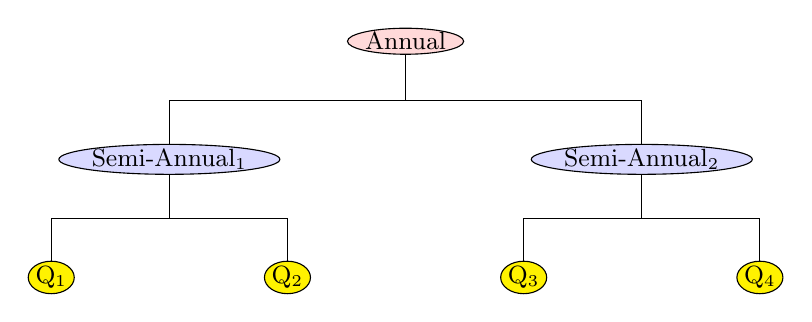
\begin{tikzpicture}
\tikzstyle{every node}=[ellipse,draw,inner sep=0.2pt,fill=red!15,font=\small]
\tikzstyle[level distance=.1cm]
\tikzstyle[sibling distance=7cm]
\tikzstyle{level 1}=[sibling distance=60mm,font=\small,set style={{every node}+=[fill=blue!15]}]
\tikzstyle{level 2}=[sibling distance=30mm,font=\small,set style={{every node}+=[fill=yellow]}]
\tikzstyle{level 3}=[sibling distance=10mm,font=\small,set style={{every node}+=[fill=green]}]
\node{Annual}[edge from parent fork down]
 child {node {Semi-Annual$_1$}
   child {node {Q$_1$}
%     child {node {M$_1$}}
%     child {node {M$_2$}}
%     child {node {M$_3$}}
   }
   child {node {Q$_2$}
%     child {node {M$_4$}}
%     child {node {M$_5$}}
%     child {node {M$_6$}}
   }
 }
 child {node {Semi-Annual$_2$}
   child {node {Q$_3$}
%     child {node {M$_7$}}
%     child {node {M$_8$}}
%     child {node {M$_9$}}
   }
   child {node {Q$_4$}
%     child {node {M$_{10}$}}
%     child {node {M$_{11}$}}
%     child {node {M$_{12}$}}
   }
 };
\end{tikzpicture}
%\end{block}
%\end{minipage}
\end{center}
\pause
\begin{alertblock}{Basic idea:}
\begin{itemize}
\item[\color{white}\ding{229}] Forecast series at each available frequency.
\item[\color{white}\ding{229}] Optimally reconcile forecasts within the same year.
\end{itemize}
\end{alertblock}
\end{frame}


\begin{frame}{Monthly series}

\only<1>{

\hspace*{-0.5cm}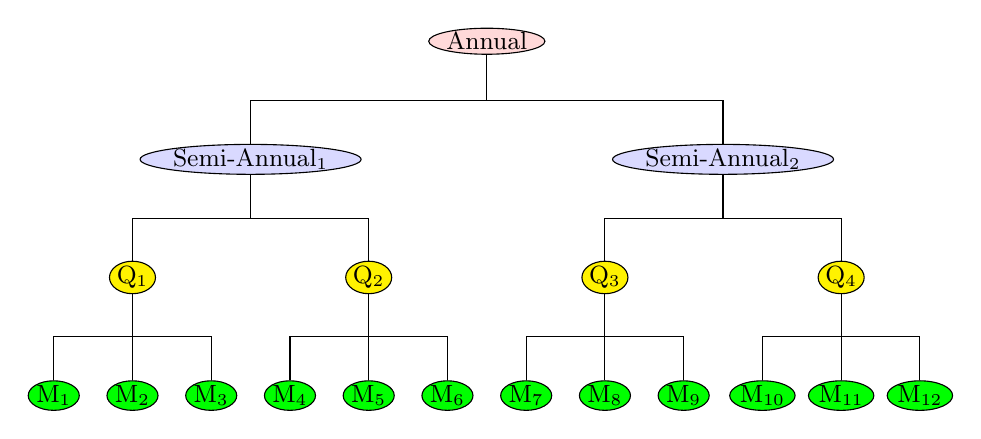
\begin{tikzpicture}
\tikzstyle{every node}=[ellipse,draw,inner sep=0.2pt,fill=red!15,font=\small]
\tikzstyle[level distance=.1cm]
\tikzstyle[sibling distance=7cm]
\tikzstyle{level 1}=[sibling distance=60mm,font=\small,set style={{every node}+=[fill=blue!15]}]
\tikzstyle{level 2}=[sibling distance=30mm,font=\small,set style={{every node}+=[fill=yellow]}]
\tikzstyle{level 3}=[sibling distance=10mm,font=\small,set style={{every node}+=[fill=green]}]
\node{Annual}[edge from parent fork down]
 child {node {Semi-Annual$_1$}
   child {node {Q$_1$}
     child {node {M$_1$}}
     child {node {M$_2$}}
     child {node {M$_3$}}
   }
   child {node {Q$_2$}
     child {node {M$_4$}}
     child {node {M$_5$}}
     child {node {M$_6$}}
   }
 }
 child {node {Semi-Annual$_2$}
   child {node {Q$_3$}
     child {node {M$_7$}}
     child {node {M$_8$}}
     child {node {M$_9$}}
   }
   child {node {Q$_4$}
     child {node {M$_{10}$}}
     child {node {M$_{11}$}}
     child {node {M$_{12}$}}
   }
 };
\end{tikzpicture}
}


\only<2->{
%\begin{minipage}{9.6cm}
%\begin{block}{}
\hspace*{-0.5cm}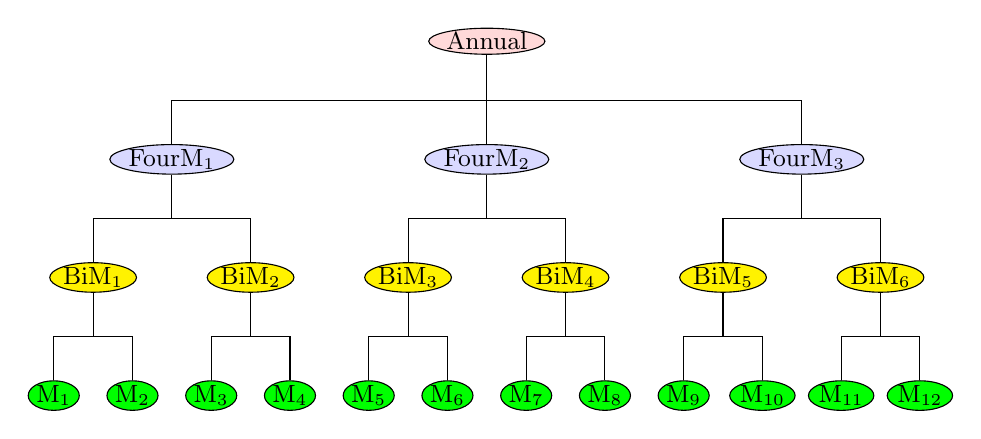
\begin{tikzpicture}
\tikzstyle{every node}=[ellipse,draw,inner sep=0.2pt,fill=red!15,font=\small]
\tikzstyle[level distance=.1cm]
\tikzstyle[sibling distance=7cm]
\tikzstyle{level 1}=[sibling distance=40mm,font=\small,set style={{every node}+=[fill=blue!15]}]
\tikzstyle{level 2}=[sibling distance=20mm,font=\small,set style={{every node}+=[fill=yellow]}]
\tikzstyle{level 3}=[sibling distance=10mm,font=\small,set style={{every node}+=[fill=green]}]
\node{Annual}[edge from parent fork down]
 child {node {FourM$_1$}
   child {node {BiM$_1$}
     child {node {M$_1$}}
     child {node {M$_2$}}
   }
   child {node {BiM$_2$}
     child {node {M$_3$}}
     child {node {M$_4$}}
   }
 }
 child {node {FourM$_2$}
   child {node {BiM$_3$}
     child {node {M$_5$}}
     child {node {M$_6$}}
   }
   child {node {BiM$_4$}
     child {node {M$_7$}}
     child {node {M$_8$}}
   }
 }
  child {node {FourM$_3$}
   child {node {BiM$_5$}
     child {node {M$_9$}}
     child {node {M$_{10}$}}
   }
   child {node {BiM$_6$}
     child {node {M$_{11}$}}
     child {node {M$_{12}$}}
   }
 };
\end{tikzpicture}
%\end{block}
%\end{minipage}
}

\vspace*{-0.4cm}


\biz
\item $k=2,4,12$ nodes
\item $k=3,6,12$ nodes
\item Why not $k=2,3,4,6,12$ nodes?
\eiz
\end{frame}


\begin{frame}{Monthly data}
\fontsize{8}{8}\sf
\hbox{${\underbrace{\footnotesize
\begin{pmatrix}
    A\\
    SemiA_{1}\\
    SemiA_{2}\\
    FourM_{1}\\
    FourM_{2}\\
    FourM_{3}\\
    Q_{1}\\
    \vdots\\
    Q_{4}\\
    BiM_{1}\\
    \vdots\\
    BiM_{6}\\
    M_{1}\\
    \vdots\\
    M_{12}
    \end{pmatrix}}_{(28\times1)}}=
    {\color{red}\underbrace{
    \footnotesize
    \begin{pmatrix}
                1 & 1 & 1 & 1 & 1~~~1~~~1~~~1 & 1 & 1& 1& 1\\
                1 & 1 & 1 & 1 & 1~~~1~~~0~~~0 & 0 & 0& 0& 0\\
                0 & 0 & 0 & 0 & 0~~~0~~~1~~~1 & 1 & 1& 1& 1\\
                1 & 1 & 1 & 1 & 0~~~0~~~0~~~0 & 0 & 0& 0& 0\\
                0 & 0 & 0 & 0 & 1~~~1~~~1~~~1 & 0 & 0& 0& 0\\
                0 & 0 & 0 & 0 & 0~~~0~~~0~~~0 & 1 & 1& 1& 1\\
                1 & 1 & 1 & 0 & 0~~~0~~~0~~~0 & 0 & 0& 0& 0\\
                  &   &   &   & \vdots        &   &  &  &  \\
                0 & 0 & 0 & 0 & 0~~~0~~~0~~~0 & 0 & 1& 1& 1\\
                1 & 1 & 0 & 0 & 0~~~0~~~0~~~0 & 0 & 0& 0& 0\\
                  &   &   &   & \vdots        &   &  &  &  \\
                0 & 0 & 0 & 0 & 0~~~0~~~0~~~0 & 0 & 0& 1& 1\\
                  &   &   &  &  &  &  &  & \\
                \phantom{\vdots}  &   &   &  & \bm{I}_{12} &  &  &  & \\
                  &   &   &  &  &  &  &  & \\
                \end{pmatrix}}_{\bS}}{\color{blue}\underbrace{\small
             \begin{pmatrix}
    M_{1}\\
    M_{2}\\
    M_{3}\\
    M_{4}\\
    M_{5}\\
    M_{6}\\
    M_{7}\\
    M_{8}\\
    M_{9}\\
    M_{10}\\
    M_{11}\\
    M_{12}\end{pmatrix}}_{\bm{b}_{t}}}$}

    \vspace*{10cm}
\end{frame}


\begin{frame}{In general}\vspace{-.3cm}

For a time series  $y_1,\dots,y_T$, observed at frequency $m$, we generate aggregate series
\begin{alertblock}{}\vspace*{-0.5cm}
$$
y_j^{\left[k\right]} = \sum^{jk}_{t=1+(j-1)k}{y_t},\qquad \text{for $j = 1,\dots,\lfloor T/k\rfloor$}
$$
\end{alertblock}
\biz
%\item For quarterly series: $k=2,4$.
%\item For monthly series: $k=2,3,4,6,12$.
\item $k \in F(m)=\{\text{factors of $m$}\}$.
\item A single unique hierarchy is only possible when there are no coprime pairs in $F(m)$.
\item $M_k=m/k$ is seasonal period of aggregated series.
%\item Remove $T-\lfloor T/m\rfloor m$ observations from beginning of sample.
\eiz
\end{frame}

% \begin{frame}{WLS weights}\vspace*{-0.2cm}\fontsize{14}{16}\sf

% \alert{Hierarchy variance scaling} $\bm{\Lambda}_H$: diagonal.

% \uncover<2->{\alert{Series variance scaling} $\bm{\Lambda}_V$: elements equal within aggregation level.}

% \uncover<3->{
% \alert{Structural scaling} $\bm{\Lambda}_S=\text{diag}(\bm{S}\bm{1})$: elements equal to \#~nodes at each level.
% \begin{itemize}
% \item Depends only on seasonal period $m$.
% \item Independent of data and model.
% \item Allows forecasts where no errors available.
% \end{itemize}}


% \begin{block}<1->{Quarterly example}\vspace*{-0.57cm}
% \begin{align*}
%   \bm{\Lambda}_H & = \diag\big(\hat{\sigma}^{2}_{A},~\hat{\sigma}^{2}_{S_1},~\hat{\sigma}^{2}_{S_2},~\hat{\sigma}^{2}_{Q_1},~\hat{\sigma}^{2}_{Q_2},~\hat{\sigma}^{2}_{Q_3},~\hat{\sigma}^{2}_{Q_4}\big) \\
%   \uncover<2->{\bm{\Lambda}_V & = \diag\big(\hat{\sigma}^{2}_A,~\hat{\sigma}^{2}_S,~\hat{\sigma}^{2}_S,~\hat{\sigma}^{2}_Q,~\hat{\sigma}^{2}_Q,~\hat{\sigma}^{2}_Q,~\hat{\sigma}^{2}_Q\big) \\}
%   \uncover<3->{\bm{\Lambda}_S & = \diag\big( 4,2,2,1,1,1,1 \big)}
% \end{align*}\vspace*{-0.9cm}
% \end{block}
% \end{frame}

\begin{frame}{\large UK Accidents and Emergency Demand}
\fullwidth{AEexample}

\begin{textblock}{12}(0.3,8.5)
\textcolor{red}{-- -- -- -- base} \hspace*{1cm}
\textcolor{blue}{\raisebox{0.5ex}{\rule{1.5cm}{1pt}} reconciled}
\end{textblock}
\end{frame}

% \begin{frame}{\large UK Accidents and Emergency Demand}\fontsize{12}{13.5}\sf
% \begin{enumerate}
% \item Type 1 Departments --- Major A\&E
% \item Type 2 Departments --- Single Specialty
% \item Type 3 Departments --- Other A\&E/Minor Injury
% \item Total Attendances
% \item Type 1 Departments --- Major A\&E $>4$ hrs
% \item Type 2 Departments --- Single Specialty $>4$ hrs
% \item Type 3 Departments --- Other A\&E/Minor Injury $>4$ \rlap{hrs}
% \item Total Attendances $>4$  hrs
% \item Emergency Admissions via Type 1 A\&E
% \item Total Emergency Admissions via A\&E
% \item Other Emergency Admissions (i.e., not via A\&E)
% \item Total Emergency Admissions
% \item Number of patients spending $>4$ hrs from decision to admission
% \end{enumerate}
% \end{frame}

% \begin{frame}{\large UK Accidents and Emergency Demand}\vspace*{-0.3cm}
% \biz
% \item \textbf{Minimum training set}: all data except the last year
% \item Base forecasts using \texttt{auto.arima()}.
% \item Reconciled using WLS$_V$.
% \item Mean Absolute Scaled Errors for 1, 4 and 13 weeks ahead using a rolling origin.
% \eiz
% \pause\fontsize{12}{14}\sf
% \begin{block}{}\centerline{
%     \begin{tabular}{lrccr}
%     \bf Aggr. Level     & $h$   & \bf Base  & \bf Reconciled & \bf Change \\
%     \midrule
%     Weekly & 1      & 1.6   & 1.3   & $-17.2\%$ \\
%     Weekly & 4      & 1.9   & 1.5   & $-18.6\%$ \\
%     Weekly & 13     & 2.3   & 1.9   & $-16.2\%$ \\
%     Weekly & 1--52  & 2.0   & 1.9   & $-5.0\%$ \\
%     Annual & 1      & 3.4   & 1.9   & $-42.9\%$
%     \end{tabular}}
%     \end{block}

% \end{frame}


% \begin{frame}{Experimental setup:}
% \biz
% \item M3 forecasting competition (Makridakis and Hibon, 2000, \textit{IJF}). In total 3003 series.
% \item 1,428 monthly series with a test sample of 12 observations each.
% \item 756 quarterly series with a test sample of 8 observations each.
% \item Forecast each series with ETS models.
% \eiz
% \end{frame}


% \begin{frame}{Results: Monthly}
% \alert{MAE percent difference relative to base}\vspace*{0.3cm}

% \tabcolsep=0.12cm
% \begin{tabular}{lrrrrrrrrr}
% \toprule
%                  & \llap{max} $h$ & BU      & WLS$_H$ & WLS$_V$ & WLS$_S$     & \\
% \midrule
% Annual           & 1   & $-19.6$ & $-22.0$ & $-22.0$ & \hl{$-25.1$}\\
% Semi-annual      & 3   & 0.6     & $-4.0$  & $-3.6$  & \hl{$-5.4$}\\
% Four-monthly     & 4   & 2.0     & $-2.4$  & $-2.2$  & \hl{$-3.0$}\\
% Quarterly        & 6   & 2.4     & $-1.6$  & $-1.7$  & \hl{$-2.8$}\\
% Bi-monthly       & 9   & 0.7     & $-2.9$  & $-3.3$  & \hl{$-4.3$}\\
% Monthly          & 18  & 0.0     & $-2.2$  & $-3.2$  & \hl{$-3.9$} \\
% %\midrule
% %\textbf{Average} &     & $-2.3$  & $-5.9$  & $-6.0$  & \hl{$-7.4$} \\
% \bottomrule
% \end{tabular}
% \vspace*{10cm}


% \end{frame}

% \begin{frame}{Results: Quarterly}
% \alert{MAE percent difference relative to base}\vspace*{0.3cm}

% \tabcolsep=0.12cm
% \begin{tabular}{lrrrrrrrrrr}
% \toprule
%                  & \llap{max} $h$ & BU      & WLS$_H$ & WLS$_V$       & WLS$_S$ \\
%  \midrule
% Annual           & 1   & $-20.9$ & -22.7   & \hl $-22.8$ & -22.7\\
% Semi-annual      & 3   & $-4.5$  & $-6.0$  & \hl $-6.2$  & -4.8 \\
% Quarterly        & 6   & 0.0     & $-0.2$  & \hl $-1.1$  & -0.3 \\
% %\midrule
% %\textbf{Average} &     & $-8.5$  & $-9.6$  & \hl{$-10.0$} & {-9.3} \\
% \bottomrule
% \end{tabular}

% \vspace*{10cm}

% \end{frame}


% \begin{frame}{thief package for R}

% \alert{\fontsize{20}{25}\sffamily \alert{thief:} \alert{T}emporal \alert{HIE}rarchical \alert{F}orecasting}\vspace*{.6cm}\pause

% \begin{block}{Install from CRAN}
%   \texttt{install.packages("thief")}
% \end{block}

% \begin{block}{Install from github}
%   \texttt{library(devtools)}\\
%   \texttt{install\_github("/robjhyndman/thief")}
% \end{block}  \pause

% \begin{alertblock}{Usage}
%   \texttt{thief(y)}
% \end{alertblock}
% % \end{frame}

% \section{Probabilistic reconciliation}

% \begin{frame}{Coherent density forecasts}

% \begin{block}{Definition: Coherence}
% Suppose $\bm{y}_t\in\mathbb{R}^n$. $\bm{y}_t$ is \emph{coherent} if $\bm{y}_t$ lies in an $m$-dimensional subspace of $\mathbb{R}^n$ spanned by the columns of the summing matrix $\bm{S}$.
% \end{block}

% \begin{block}{Definition: Coherent density forecasts}
% Any density $p(\bm{y}_{t+h})$ such that $p(\bm{y}_{t+h})=0$ for all $\bm{y}_{t+h}$ in the null space of $\bm{S}$.
% \end{block}\pause

% \begin{itemize}
%   \item Coherent point forecasts: $\tilde{\bm{y}}_{T+h|T} = \bm{S}\bm{P}\hat{\bm{y}}_{T+h}$.
%   \item Coherent variance forecasts (assuming unbiasedness):
%   $\tilde{\bm{\Sigma}}_{T+h} = \bm{S}\bm{P}\hat{\bm{\Sigma}}_{T+h}\bm{P}'\bm{S}'$
% \end{itemize}

% \end{frame}

% \begin{frame}{Coherent Gaussian forecasts}\fontsize{14}{16}\sf
% \begin{alertblock}{}
% \centerline{$\bm{y}_{T+h|T} \sim N(\tilde{\bm{y}}_{T+h|T}, \tilde{\bm{\Sigma}}_{T+h})$}
% \end{alertblock}

% Let $L$ be the Energy Score (a proper scoring rule):
% \begin{block}{}\fontsize{14}{14}\sf
% \centerline{$L(\tilde{\bm{Y}}_{T+h}, \bm{y}_{T+h}) = \text{E}\| \tilde{\bm{Y}}_{T+h} - \bm{y}_{T+h} \|^\alpha\textstyle
% - \frac{1}{2}\text{E}\| \tilde{\bm{Y}}_{T+h} - \tilde{\bm{Y}}_{T+h}' \|^\alpha$}
% for $\alpha \in (0,2]$, where $\tilde{\bm{Y}}_{T+h}$ and $\tilde{\bm{Y}}_{T+h}'$ are independent rvs from $N(\tilde{\bm{y}}_{T+h|T}, \tilde{\bm{\Sigma}}_{T+h})$.
% \end{block}

% \begin{itemize}
%   \item There is no closed form expression for $L(\tilde{\bm{Y}}_{T+h}, \bm{y}_{T+h})$ for $\alpha \in (0,2)$ under the Gaussian predictive distribution.
% \item When $\alpha=2$,  $L(\tilde{\bm{Y}}_{T+h}, \bm{y}_{T+h}) = \| \tilde{Y}_{T+h} - \bm{y}_{T+h} \|^2$
% \item This is equivalent to MinT solution.
% \end{itemize}
% \end{frame}

% \begin{frame}{Coherent nonparametric forecasts}

% \begin{enumerate}
% \item  Simulate forecast distributions at each bottom level node using univariate models
% \item Compute empirical copulas for each parent+children group.
% \end{enumerate}

% \pause

% \begin{itemize}
%   \item Equivalent to ``bottom-up'' point forecasting. No reconciliation involved.
%   \item Successfully applied to forecasting smart-metre electricity demand (Ben Taieb, Taylor, Hyndman, 2017)
% \end{itemize}
% \end{frame}


\begin{frame}{Papers and packages}

\begin{tabular}{lp{8.7cm}}
\raisebox{-1.6cm}{
\includegraphics[width=1.4cm]{EJOR}} & \RaggedRight Athanasopoulos, Hyndman, Kourentzes \& Petropoulos (2017) Forecasting with temporal hierarchies. \emph{EJOR}, \textbf{262}(1) 60--74.\\[0.3cm]
\raisebox{-.9cm}{
\includegraphics[width=1.4cm]{Rlogo}} & \RaggedRight Hyndman \& Kourentzes (2017). \textbf{thief}: Temporal HIErarchical Forecasting \par
  \url{pkg.robjhyndman.me/thief/}
\end{tabular}

\vspace*{10cm}

\begin{textblock}{6.6}(3.05,7.6)
\begin{alertblock}{}
Papers, packages and slides available at \textbf{robjhyndman.com}
\end{alertblock}
\end{textblock}

\end{frame}


\end{document}


